\newcommand{\app}{\raise.17ex\hbox{$\scriptstyle\sim$}}
\newcommand{\ncdot}{{\mkern 0mu\cdot\mkern 0mu}}
\def\x{\times}

\newcolumntype{x}[1]{>{\centering\arraybackslash}p{#1pt}}
\newcommand{\dt}[1]{\fontsize{8pt}{.1em}\selectfont \emph{#1}}
\newlength\savewidth\newcommand\shline{\noalign{\global\savewidth\arrayrulewidth
  \global\arrayrulewidth 1pt}\hline\noalign{\global\arrayrulewidth\savewidth}}
\newcommand{\tablestyle}[2]{\setlength{\tabcolsep}{#1}\renewcommand{\arraystretch}{#2}\centering\footnotesize}
\makeatletter\renewcommand\paragraph{\@startsection{paragraph}{4}{\z@}
  {.5em \@plus1ex \@minus.2ex}{-.5em}{\normalfont\normalsize\bfseries}}\makeatother

\xjtuappendixchapter{外文文献翻译}

\begin{center}
    \sihao\textbf{Mask R-CNN:用于预测遮罩的区域卷积神经网络}
\end{center}

\textbf{摘要}:我们展现了一个概念意义上简单、稳定以及通用的目标实例划分框架。我们的方法能够高效地检测图片中目标,与此同时还能为目标实例生成高质量的划分遮罩。我们的方法在Faster R-CNN的基础上,增加了一条用于预测目标物体遮罩的分支,与现存的预测目标物体边界框的分支\emph{并行}。我们将此方法称为Mask R-CNN。Mask R-CNN训练简单,且仅比处理帧速为5fps的Faster R-CNN增加了少量的运算量。不仅如此,在Mask R-CNN框架上增加其它的任务也十分简单,例如允许我们在相同的框架下估计人物的姿势。我们的方法在COCO系列挑战中的三个任务都取得了最佳成绩,包括实例分割、边界框目标检测以及人体姿态检测。在没有使用调参技巧的情况下,Mask R-CNN超过了每个任务中所有现存的单一模型框架,包括COCO 2016挑战的冠军。我们希望我们的模型能够成为一个坚实的基础模型,为今后实例级别的识别研究减轻负担。本框架的源代码已经公开在:\url{https://github.com/facebookresearch/Detectron}.

\xjtuappendixsection{引言}
在过去很短的时间内,计算机视觉社区快速地提高了目标检测和语义分割的结果。在很大的程度上,一些强大的基础模型驱动了这些结果,例如用于目标检测任务的Fast/Faster R-CNN 框架以及用于语义分割的全卷积网络(FCN)框架。这些方法的概念很新颖,在提供了灵活性和稳健性的同时,也提供了快速的训练和检测。我们本次工作的目标是开发一个同等有效的\emph{实例分割}框架。

\begin{figure}
\begin{minipage}{0.35\textwidth}
  \centering
  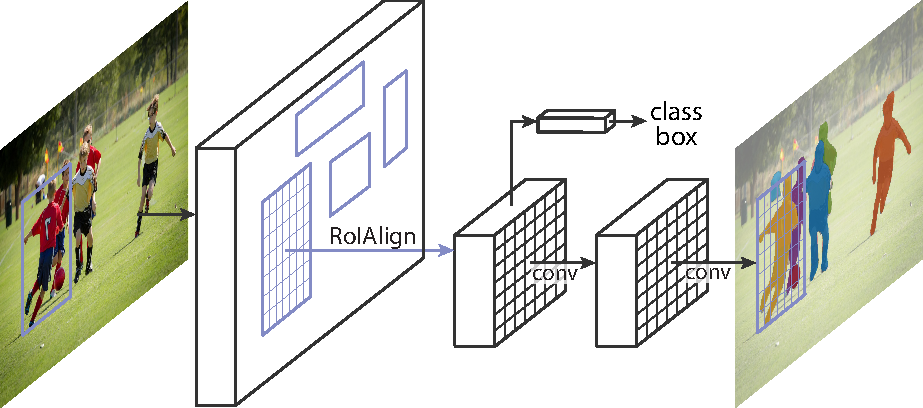
\includegraphics[width=1\linewidth]{figures/mask_rcnn/teaser}\vspace{2mm}
  \caption{用于实例分割的\textbf{Mask\hspace{0.1297em}R-CNN}框架。}
  \label{fig:teaser}
\end{minipage}\hspace{1.5em}
\begin{minipage}{0.6\textwidth}
  \begin{minipage}{0.365\linewidth}
  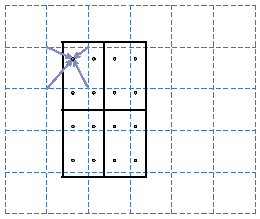
\includegraphics[width=\textwidth,trim={0 0 7.5mm 0},clip]{figures/mask_rcnn/roialign}
  \end{minipage}\hspace{0.5em}
  \begin{minipage}{0.605\linewidth}
  \caption{\textbf{RoIAlign:} 虚线网格表示特征图,实线表示 RoI(在这个例子里面包含$2\times2$的容器),容器中的点表示每个容器中的4个采样点。RoIAlign通过特征图上附近网格点的双线性插值计算每个采样点的值。 在 RoI 内部,其容器或采样点中涉及的任何坐标都不执行量化。}
  \label{fig:roialign}
  \end{minipage}
\end{minipage}
\end{figure}

实例分割非常具有挑战性,因为它需要在正确地检测出一张图片中所有目标的同时,精确地划分每一个实例物体。因此实例分割问题包含了传统计算机视觉领域中的\emph{目标检测}和\emph{语义分割}任务。其中目标检测的任务是对于图片中的每一个目标进行分类,并使用边界框定位目标。而语义分割的目标是将图片中的每一个像素分类为一些固定的类别,而不区分每一个目标实例。\footnote{我们使用术语\emph{目标检测}表示检测目标的边界框,而不是遮罩;使用术语\emph{语义分割}表示将每一个像素分类而不区分目标实例,与通用的术语一致。同时我们使用术语\emph{实例分割}来表示既包含语义分割也包含目标检测的任务。} 对于实例分割任务,有人可能会认为需要一个复杂的方法才能得到好的结果。然而我们展示了一个极其简单、灵活以及快速的系统,能够超越先前在实例分割领域最先进的成果。

我们这个称为\emph{Mask R-CNN}的方法是Faster R-CNN的扩展,增加了一个用于预测每一个感兴趣区域(Region of Interest,RoI)的分割遮罩的分支,该分支与现有的用于分类及边界框回归的分支\emph{并行}(图~\ref{fig:teaser})。该遮罩分支是一个应用于每一个感兴趣区域的全连接卷积网络,用于像素到像素级别的分割遮罩预测。Faster R-CNN框架便于用很多种灵活的架构设计实现,对于一个特定的Faster R-CNN网络,基于此的Mask R-CNN模型很也容易实现和训练。不仅如此,遮罩分支仅增加了少量的计算量,使得一个快速的系统和实验成为可能。

Mask R-CNN的原则是作为Faster R-CNN的一个直观的扩展框架,然而正确地构造遮罩分支是取得好结果的关键。更重要的是,Faster R-CNN不是为在输入和输出之间像素到像素对齐而设计的。这种设计在\emph{RoIPool}运用粗粒度的空间量化进行特征提取时最为明显。其中RoIPool是\emph{事实上的}处理实例的核心操作。为了解决不对齐的问题,我们提出了简单、免量化的层,称为\emph{RoIAlign},其完整地保留了额外的空间位置。尽管这看上去是一个很小的改变,然而具有很大的影响:它将遮罩预测的准确率相对提升了10\%到50\%,并且在更严格的评估方式下提升更明显。我们的第二个发现是,有必要将遮罩预测与分类预测\emph{解耦}:我们独立地对每个类别进行二元遮罩预测,取消了不同类别之间的竞争,同时利用网络中RoI分类分支进行类别预测。与之相反的,全卷积网络通常用于对每个像素进行多分类操作,该操作将分割与分类耦合起来,这样的传统方法在我们的实验的实例分割任务中表现不佳。

在没有使用任何调参技巧的情况下,Mask R-CNN的表现超过了所有先前在COCO实例分割任务中最优秀的单模型的结果,包括依靠高度工程化技巧赢得2016年挑战的冠军。作为一个附带的结果,我们的方法在COCO目标检测任务中依然表现出色。在控制变量分析对比实验中,我们评估了模型中多个基本的组成部分,这让我们能够评估模型的稳健性以及分析核心元素的影响。

我们的模型在单张GPU上每一帧的运行时间大约为200毫秒,在一台拥有8张GPU的机器上使用COCO数据集进行训练大约需要花费两天。我们相信如此快的训练和测试速度,以及模型的灵活性和准确性,能够让今后的实例分割研究获益。

最后,我们通过利用COCO姿势关键点数据库完成人类姿势估计任务简单展示了该框架的通用性。通过将每一个关键点看作是一个有固定个数1的二元遮罩,再加上一些很小的修改,就可以将原始的Mask R-CNN框架应用于检测每一个人物实例的姿势。在没有任何调参技巧的情况下,Mask R-CNN的表现超过了COCO 2016人体姿态关键点挑战的获胜者,同时检测速度依然是每秒5帧。因此Mask R-CNN可以更宽泛地看作是一个用于\emph{实例级别}的识别的灵活框架,并且可以很轻易地扩展到其它的复杂任务当中。

我们已经将源代码公开以促进今后的研究工作。

\xjtuappendixsection{相关工作}

\paragraph{R-CNN:} 基于区域的卷积神经网络(Region-based CNN,R-CNN)这样的用于边界框目标检测的方法,通常被用于处理大量的目标候选区域,同时独立地在每一个RoI上评估卷积网络。在2014年,经过扩展的R-CNN可通过RoIPool用于处理在特征图上的RoI,使其取得更高的准确率和更快的速度。Faster R-CNN再度扩展了此项工作,其使用区域候选网络(Region Proposal Network,RPN)来学习注意力机制。Faster R-CNN相比于之后的改进模型更加灵活和稳健 ,同时其依然是当前多个评估标准中领先的框架。

\paragraph{实例分割:} 受R-CNN良好效果的影响,很多实例分割的方法都是基于\emph{分割候选物}的。先前的方法  都采取的是自下而上的分割形式 . DeepMask  以及接下来的工作  会通过学习生成分割形状的候选,这些候选将使用Fast R-CNN进行分类。在这些方法中,形状的分割\emph{先于}目标的识别,这种做法不仅速度慢,而且精度低。类似地,戴先生等人  提出了一个复杂的多级级联,该方法在分类之后使用候选的边界框来预测候选的分割形状。与此相反,我们的方法基于\emph{并行的}遮罩和类别预测任务,使得该方法更加简单和灵活。

最近,李先生等人  将中的候选分割形状系统与中的目标检测系统结合起来,用于 ``全卷积实例分割'' (fully convolutional instance segmentation,FCIS)。 在  当中的基本想法是预测一系列全卷积的且位置敏感的输出通道。这些通道可同时呈现目标类别、边界框以及遮罩信息,使得系统更快。但是 FCIS 也暴露了其在重叠的实例上会出现系统性的错误,以及会生成一些假的遮罩边缘(见图~\ref{fig:results_vs_fcis}),这表明了在实例分割问题上存在根本性的困难,极具挑战性。

其它形式的实例分割解决方案  是由语义分割问题的解决来驱动的。由每一个像素的分类结果出发(例如FCN的输出),这些方法尝试将同一个类别的像素分割为不同的实例。与这些方法中\emph{分割优先}策略相反,Mask R-CNN基于\emph{实例优先}的策略。我们期待在今后的研究中,两种策略可以更进一步地融合。

\xjtuappendixsection{Mask R-CNN}\label{sec:maskR-CNN}

Mask R-CNN 在概念上很简洁:Faster R-CNN对于每个候选的目标会有两个输出,一个是目标的分类标签,另一个是目标的边界框。基于此我们增加了第三个分支,用于输出目标的遮罩。因此Mask R-CNN是一个自然而直观的想法。然而增加的遮罩输出与类别标签和边界框输出不同,需要获取一个目标更\emph{细致}的空间分布信息。接下来我们将介绍Mask R-CNN的关键元素,这些元素是Fast/Faster R-CNN所缺少的。

\paragraph{Faster R-CNN:} 我们首先简单回顾一下Faster R-CNN检测器 。Faster R-CNN 包含两个阶段。第一个阶段称为区域候选网络(Region Proposal Network,RPN),该阶段生成候选的目标边界框。第二个阶段本质上是一个Fast R-CNN 模型, 该阶段使用RoIPool从每一个候选框中提取特征,将这些特征用于分类和边界框回归。两个阶段使用的特征可以共享,以此来加速检测的速度。我们建议读者阅读以了解Faster R-CNN与其它框架最新的、最全面的对比。

\paragraph{Mask R-CNN:} Mask R-CNN同样包含两个阶段的过程,并且第一阶段(RPN)没有改动。在第二阶段,在\emph{并行}地预测类别标签和边界框两条分支的同时,Mask R-CNN对于每一个RoI还输出了一个二元的遮罩。这与最近出现的系统相反,在那些系统中分类\emph{独立于}遮罩预测(例如 )。我们的方法继承Fast R-CNN 的精神,将边界框的分类和回归\emph{并行}执行,这种精神已经被证实大量简化了原始的R-CNN 中多阶段流水线过程。

形式化的表述是,在训练阶段,我们在每一个采样的RoI上定义了一个多任务的损失函数,该损失函数表示为$L = L_{cls} + L_{box} + L_{mask}$。其中分类损失 $L_{cls}$ 和边界框损失 $L_{box}$ 与当中的定义相一致。遮罩分支对于每一个RoI都有一个$Km^2$维的输出,该输出由$K$个分辨率为$m \times m$的二元遮罩组成,每一个遮罩对应于$K$个类别当中的一个类别。为了达到这样的目标,我们对每一个像素都使用了sigmoid函数激活,同时定义$L_{mask}$为平均二元交叉熵损失。对于真实分类标签为$k$的RoI,$L_{mask}$只由第$k$个遮罩定义(输出的其它遮罩不参与损失的计算)。

我们这样定义的 $L_{mask}$ 允许网络为每一个类别都生成一个遮罩,避免了不同类别之间遮罩的影响。我们依赖一个独立的分类分支来预测分类,分类结果用于从遮罩输出当中选择一个。这样使得遮罩分支与分类分支\emph{解耦}。与通常的实践不同得是,在通常的实践中,FCN会被用于语义分割,且通常会使用针对每一个像素的\emph{sigmoid}函数,以及\emph{多项的}交叉熵损失。在这样的情况下,不同类别的遮罩会存在冲突,而在我们的方法中不会这样,因为我们使用了针对每一个像素的 \emph{sigmoid}函数以及\emph{二元}损失。我们通过实验证明了这样的形式是我们取得好的实例分割结果的关键。

\paragraph{遮罩的表示:} 一个遮罩编码了一个输入目标的\emph{空间上的}布局。因此,不像类别标签以及边界框这样必须通过全连接层(\emph{fc})降维成短向量,提取遮罩的空间结构可以很自然地想到利用卷积来表达像素到像素之间的相关性。

特别地,我们使用 FCN  对于每一个RoI预测了一个尺寸为$m \times m$的遮罩。这使得遮罩分支内的每一层保留明确的$m \times m$的目标物体空间布局,而非将其折叠成一个缺少空间信息的向量。与先前采取全连接(\emph{fc})层来预测遮罩的方法 ,我们的全卷积表示需要的参数更少,并且实验表明这样的准确率更高。

这种像素到像素的行为要求我们的 RoI 特征(它们本身就是小特征图)能够很好地对齐,从而忠实地保留显式的每像素空间相关性。这促使我们开发了以下 \emph{RoIAlign} 层,该层在遮罩预测中发挥关键作用。

\paragraph{RoIAlign:} RoIPool  是从每个 RoI 中提取一个小特征图(例如~$7\times7$)的标准操作。 RoIPool 首先将由浮点数构成的RoI\emph{量化}为离散粒度的特征图,然后将该量化的RoI划分为自身量化的空间容器,最后聚合每个容器所涵盖的特征值(通常通过最大池化)。例如对于连续坐标 $x$, 量化是通过计算 $x / 16$来执行的,其中 16 是特征图的步长,$[\cdot]$是舍入;同样地,当划分容器(例如~$7\times7$)时执行的也是量化。 这些量化引入了 RoI 和提取的特征之间的错位。 虽然这可能不会影响分类,这对于小型的转换很有用,但它对预测精确到像素级别的遮罩有很大的负面影响。

为了解决这个问题,我们提出一个\emph{RoIlign}层,其去除了RoIPool层的严格量化,正确地将提取的特征与输入\emph{对齐}。 我们提出的修改很简单:我们避免任何RoI边界或容器的量化(例如,我们使用$x/16$而不是$[x/16]$)。 我们使用双线性插值计算每个RoI容器中四个常规采样位置的输入特征的精确值,并汇总结果(使用最大值或平均值),详细信息请参见图\ref{fig:roialign}。我们注意到,结果对精确的采样位置,或者对有多少个点进行采样不敏感,\emph{只要}不进行量化即可。

正如我们在\S 附录\ref{sec:ablations}中所示,RoIAlign可以带来很大的改进。我们也比较了RoIWarp提出的操作。与RoIAlign不同,RoIWarp忽略了对齐问题,并像RoIPool一样实现了量化RoI。因此,尽管RoIWarp也采用了双线性重采样,但它的性能与RoIPool相当(如表\ref{tab:ablation:roialign}所示),证明了对齐的关键作用。

\paragraph{网络体系结构:} 为了演示我们方法的一般性,我们实例化了具有多种体系结构的Mask R-CNN。为了清楚起见,我们区分:(i)用于整个图像上的特征提取的卷积\emph{主干}体系结构,以及(ii)用于边界框识别(分类和回归)的网络\emph{前部}和分别应用于每个RoI的遮罩预测。

我们用术语\emph{网络深度特征}来表示主干体系结构。 我们评估深度为50或101层的ResNet和ResNeXt 网络。带有ResNet的Faster R-CNN的最初实现从第四阶段的最后卷积层提取特征,我们称之为C4。 例如,ResNet-50 的主干用 ResNet-50-C4 表示。 这是一个常用的表示选择和表示方式。

我们还探索了林先生等人最近提出的另一种更有效的主干网络,称为特征金字塔网络(Feature Pyramid Network,FPN)。 FPN 使用具有横向连接的自顶向下架构从单一比例输入构建网络内特征金字塔。以FPN为主干的Faster R-CNN根据其规模从不同层次的特征金字塔中提取 RoI 特征,但其他方法与 vanilla ResNet 类似。以ResNet-FPN为主干的Mask R-CNN进行特征提取可以提高精度和速度。有关FPN的更多详细信息,请读者参阅相关文献。

对于网络的\emph{前部},我们大部分沿用以前工作中提出的架构,并在其中添加全卷积遮罩预测分支。具体来说,我们根据ResNet和FPN论文扩展了Faster R-CNN的前部。 详细信息如图\ref{fig:head}所示。 ResNet-C4主干的前部包括计算密集的ResNet第5阶段(即9层的`res5')。对于FPN,主干已经包含 res5,因此允许使用更少卷积核的更高效的前部。

我们注意到我们的遮罩分支有一个简单的结构。更复杂的设计有提高性能的潜力,但不是这项工作的重点。

\begin{figure}[t]
\centering
\begin{overpic}[width=1.0\linewidth]{figures/mask_rcnn/head}
 \put(33,29){Faster R-CNN}
 \put(33,26){w/ ResNet }
 \put(84,29){Faster R-CNN}
 \put(84,26){w/ FPN }
\end{overpic}
\caption{\textbf{前部体系结构}: 我们扩展了两个现有的Faster R-CNN的前部。 左图和右图分别显示ResNet C4和FPN主干的前部,其都添加了遮罩分支。数字表示空间分辨率和通道数。箭头表示可以从上下文中推断出的卷积层、反卷积层或者全连接层(卷积层会保留空间维度,而反卷积层会增加空间维度)。除了输出卷积层的尺寸为$1\times1$,所有的卷积核的尺寸都是$3\times3$。反卷积核尺寸为$2\times2$且步长为2,同时我们在隐藏层中使用了ReLU。 \emph{左}:`res5'表示ResNet的第五阶段,为了简单起见,我们进行了更改,使得第一个卷积核以步长1在尺寸为$7\times7$的RoI上操作,(而不是以步长2在尺寸为$14\times14$RoI上)。\emph{右}:$\times4$表示一连串的四次转换。}
\label{fig:head}
\end{figure}

\xjtuappendixsubsection{实现细节}\label{sec:impl}

我们根据现有的Fast/Faster R-CNN工作来设置超参数。尽管这些超参数的设置是针对原始论文中的目标检测任务而做出的,但我们发现这些设置对于我们的实例分割任务也是健壮的。

\paragraph{训练:} 与Fast R-CNN一样,如果RoI的与真实边界框的IoU大于或等于0.5,则RoI被认为是正确的,否则为错误的。遮罩损失$L_{mask}$仅在正确的RoI上定义。遮罩的目标输出是正确的RoI与其关联的实际遮罩之间的交集。

\begin{figure*}[t]
\centering
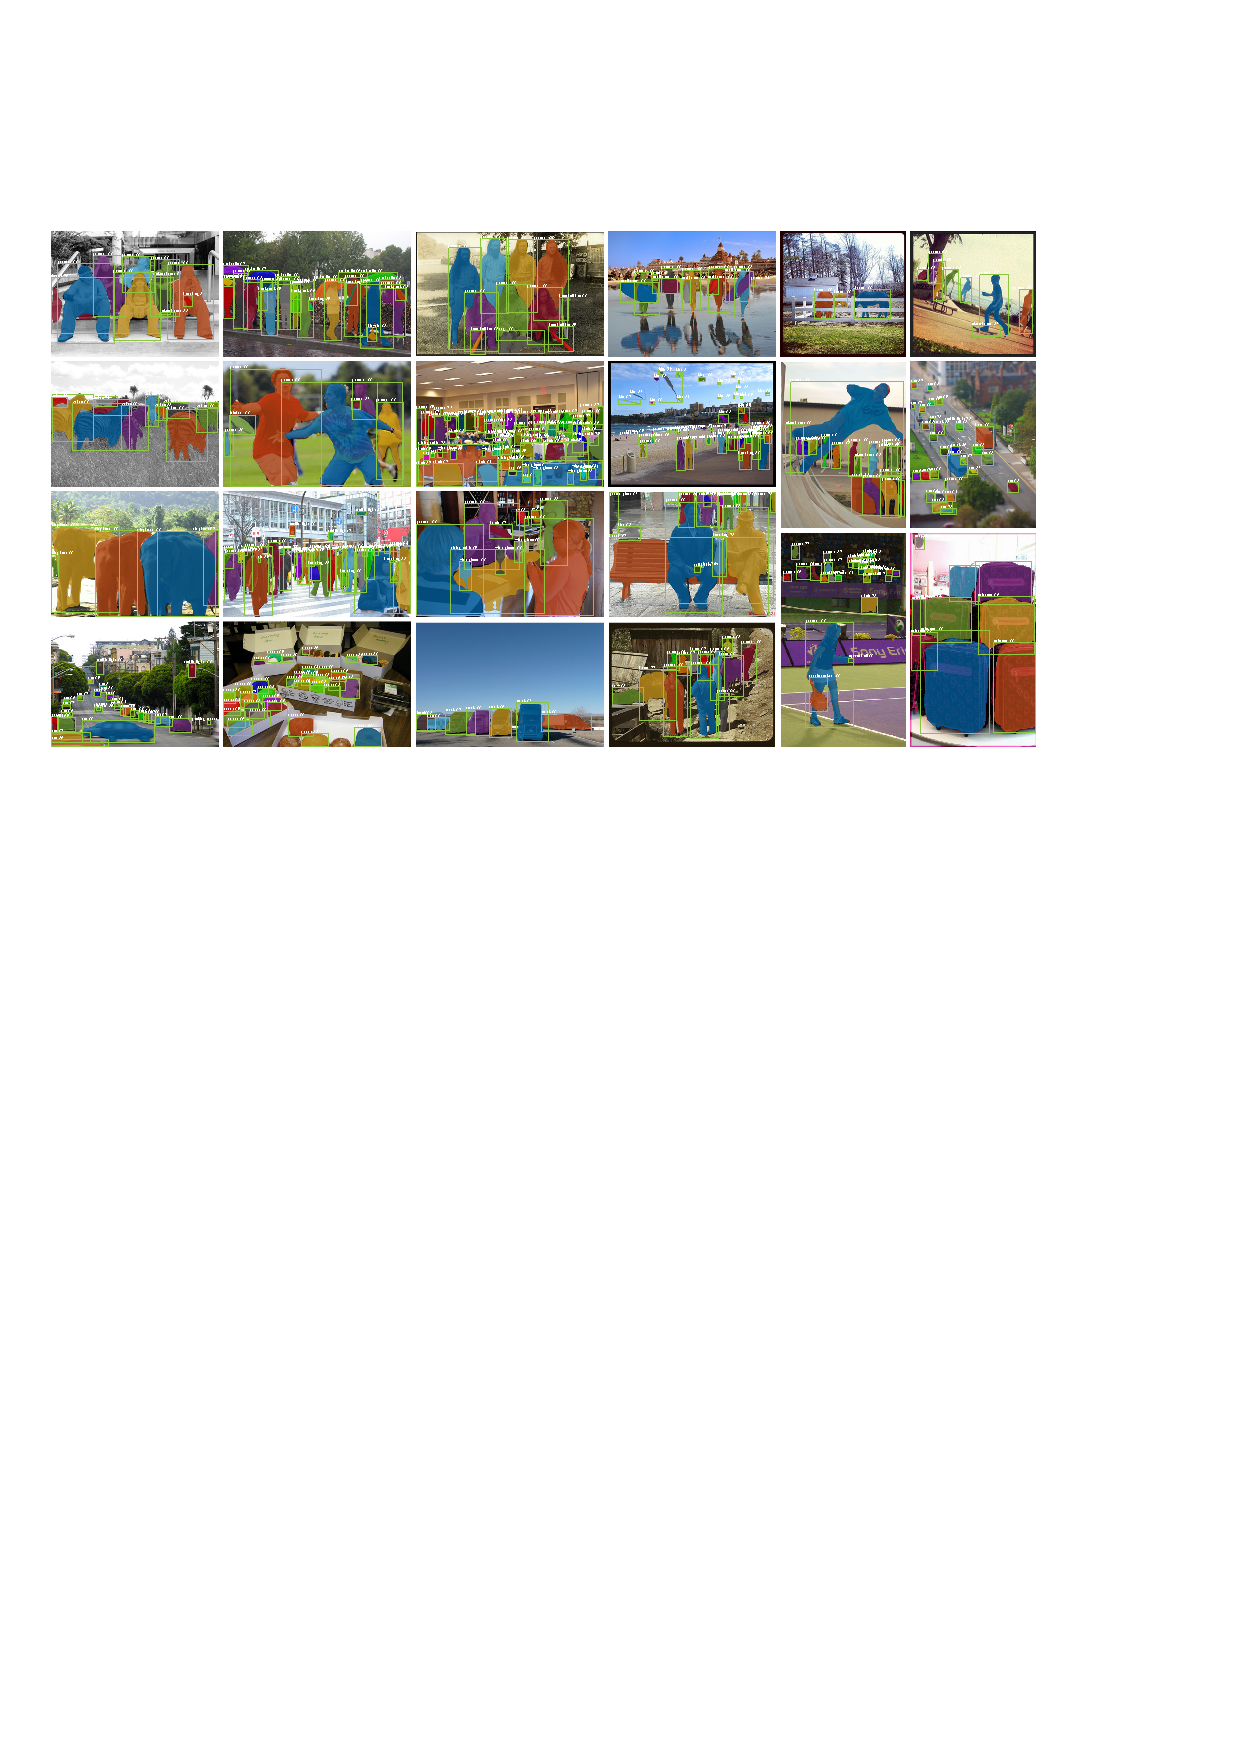
\includegraphics[width=1.0\linewidth]{figures/mask_rcnn/results_more}
\caption{\textbf{Mask R-CNN}在COCO测试集上的更多结果。取得该结果的模型使用了ResNet-101-FPN作为主干,速度为5fps,遮罩平均精度为35.7(见表\ref{tab:final_mask})。}
\label{fig:results_more}
\end{figure*}

\begin{table*}[t]
\tablestyle{3.5pt}{1.1}
\begin{tabular}{l|l|x{22}x{22}x{22}|x{22}x{22}x{22}}
 & backbone &  AP &  AP$_{50}$ & AP$_{75}$ & AP$_S$ &  AP$_M$ &  AP$_L$\\
\shline
 MNC  & ResNet-101-C4
  & 24.6 & 44.3 & 24.8 & 4.7 & 25.9 & 43.6\\
 FCIS  +OHEM & ResNet-101-C5-dilated
  & 29.2 & 49.5 & - & 7.1 & 31.3 & 50.0\\
 FCIS+++  +OHEM & ResNet-101-C5-dilated
  & 33.6 & 54.5 & - & - & - & -\\
\hline
 \textbf{Mask R-CNN} & ResNet-101-C4
  & 33.1 & 54.9 & 34.8 & 12.1 & 35.6 & 51.1 \\
 \textbf{Mask R-CNN} & ResNet-101-FPN
  & 35.7 & 58.0 & 37.8 & 15.5 & 38.1 & 52.4\\
 \textbf{Mask R-CNN} & ResNeXt-101-FPN
  & \textbf{37.1} & \textbf{60.0} & \textbf{39.4} & \textbf{16.9} & \textbf{39.9} & \textbf{53.5}
\end{tabular}
\caption{\textbf{实例分割} 在COCO\texttt{test-dev}数据集上的\emph{遮罩}平均精度. MNC和FCIS分别是2015年和2016年COCO实例分割挑战的获胜者。在没有任何调参技巧的情况下,Mask R-CNN的表现超过了更复杂的FCIS+++模型,该模型包括了多尺度训练、测试,水平平移测试,以及OHEM。所有的图片都是\emph{单一模型}下的结果。}
\label{tab:final_mask}
\end{table*}

我们采用图像中心训练。调整图像大小以使其长、宽中较短的一边为800像素。每个最小批量在每个GPU上有2张图像,每个图像都有$N$个抽样的RoI,比例为1:3。在C4主干下,$N$为64,在FPN主干下,$N$为512。我们在8个GPU上进行训练(因此有效的最小批量为16),进行16万次迭代,学习率为0.02,在迭代12万次时减少为原来的$1/10$。我们使用0.0001作为重量衰减以及0.9作为动量。在使用使用ResNeXt时,我们每个GPU训练1个图像并进行相同次数的迭代,初始学习率为0.01。

RPN锚点(anchors)跨越5个尺度和3个纵横比。为了方便控制变量,除非另有说明,否则RPN将单独进行训练并且不与Mask R-CNN共享特征。对于本文中的每个部分,RPN和Mask R-CNN具有相同的主干,因此它们的参数可以共享。

\paragraph{预测:} 在测试时,以C4为的候选框个数为300,以FPN为主干的候选框个数为1000。我们将这些候选框分别送入边界框预测分支,然后进行非最大抑制。然后将得分最高的100个检测框输入遮罩分支。虽然这与训练中使用的并行计算不同,但它加快了预测速度并提高了准确性(因为使用了更少,更准确的RoI)。遮罩分支对于每个RoI可以预测$k$个遮罩,但我们只使用第$k$个遮罩,其中$k$是分类分支预测的类别。然后将尺寸为$m\times m$的浮点数遮罩输出调整为RoI的大小,并使用阈值0.5将其二值化。

请注意,由于我们仅在前100个检测框中计算掩码,因此Mask R-CNN相对其对应的Faster R-CNN模型进增加了一个很小的开销(例如在典型模型上大约为20\%)。

\xjtuappendixsection{实验:实例分割}\label{sec:results}

我们在COCO数据集上以控制变量的方式,将Mask R-CNN与对应领域最先进的模型进行了彻底的比较。我们展示COCO数据集上常规的指标,包括平均精度(AP,在IoU阈值以上的均值),$AP_{50}$,$AP_{75}$和$AP_S$,$AP_M$,$AP_L$(不同AP规模)。除非另有说明,AP将使用\emph{遮罩}IoU进行评估。与以前的工作一样,我们使用8万张训练图像和3.5万张验证集子集图像(\texttt{trainval35k})进行训练,并展示剩余的5千张验证集图像(\texttt{minival})上的控制变量实验。我们还展示了\texttt{test-dev}测试集上的结果。

\xjtuappendixsubsection{主要结果}

\begin{figure*}[t]
\centering
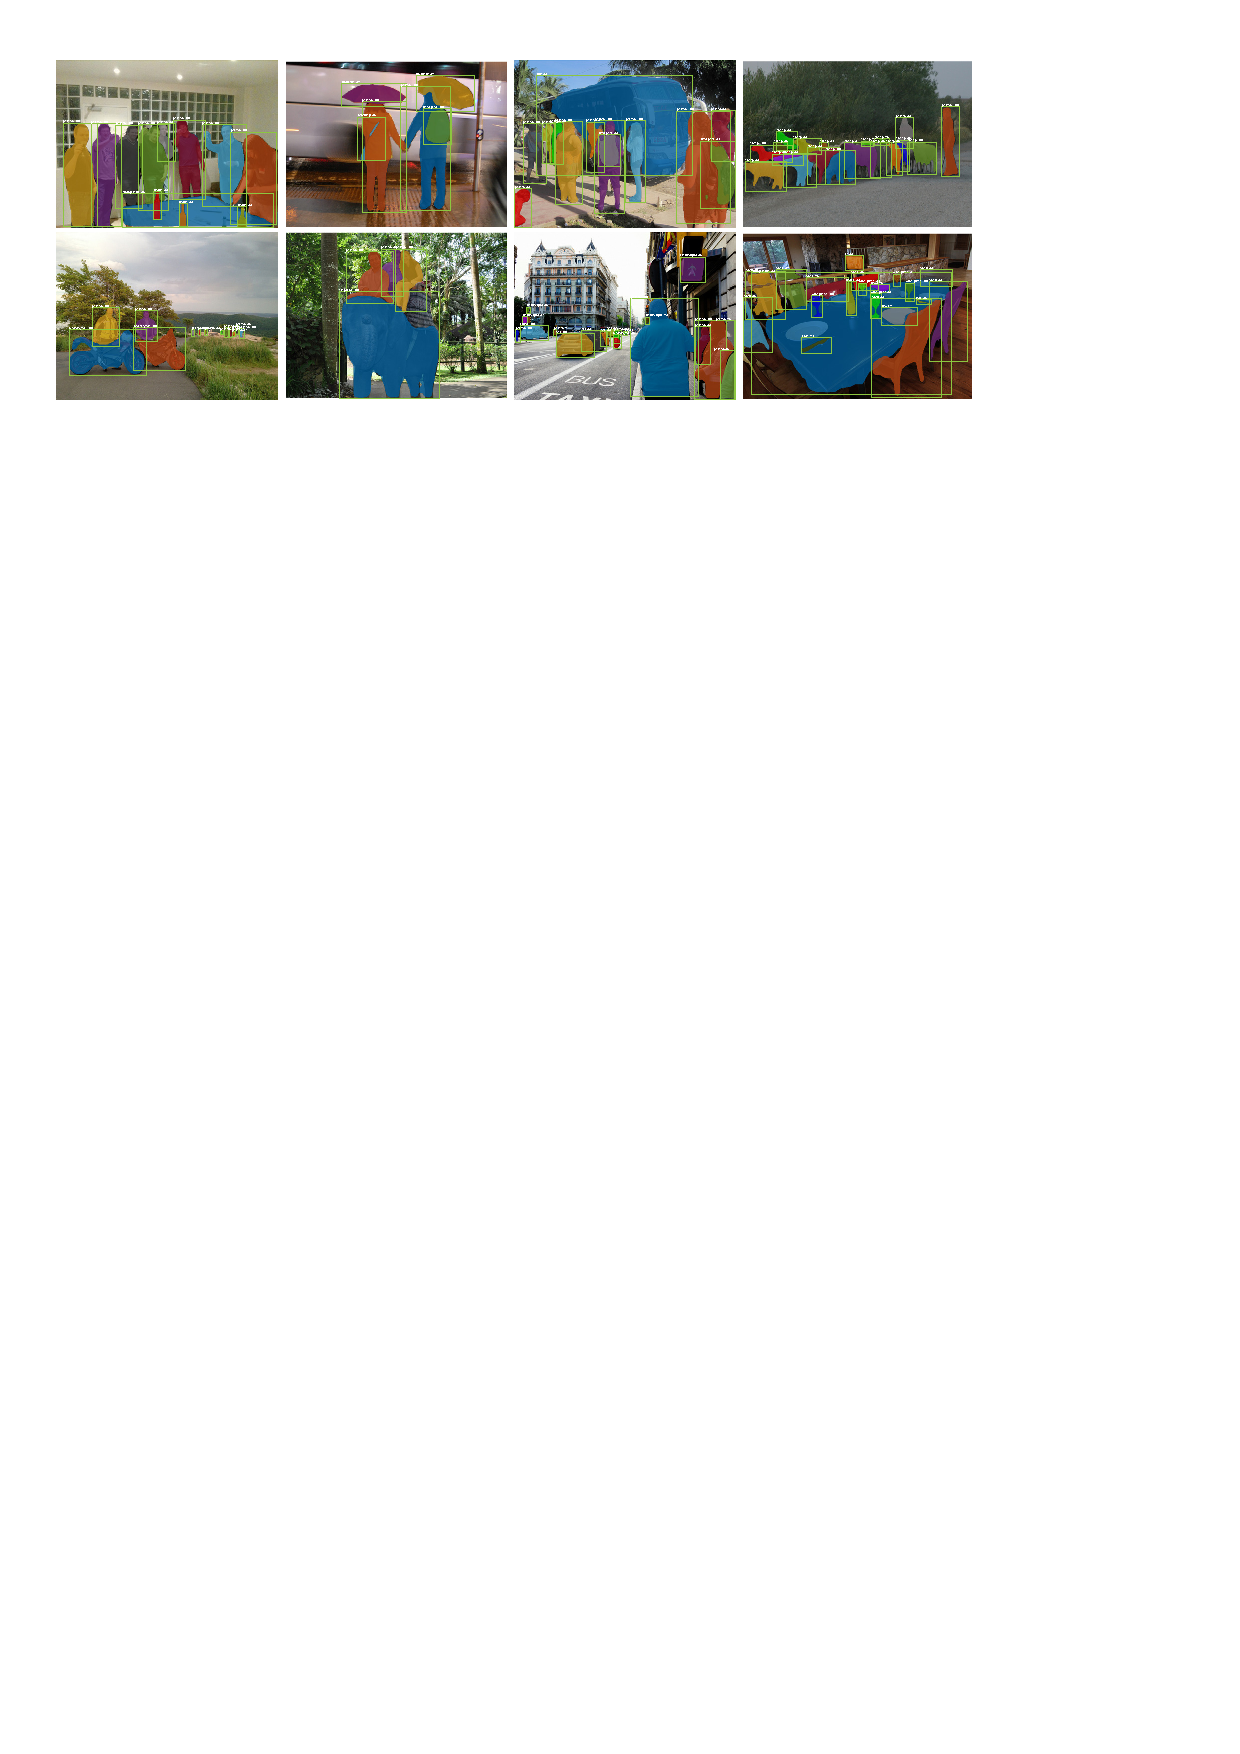
\includegraphics[width=1\linewidth]{figures/mask_rcnn/results_main}
\caption{\textbf{Mask R-CNN}框架在COCO测试集上的结果。这些结果基于ResNet-101  模型,达到了35.7的\emph{遮罩}准确率,且运行速度为每秒5帧. 遮罩使用了不同的颜色来展示。图中同样展示了边界框、类别名称以及置信度。}
\label{fig:results_main}\vspace{-2mm}
\end{figure*}

我们将Mask R-CNN与最先进的实例分割模型进行比较,结果如图\ref{tab:final_mask}。我们模型的所有实例都优于先前最先进的模型的基础变体。这包括MNC和FCIS,它们分别是2015年和2016年的分类挑战的获胜者。以ResNet-101-FPN为主干的Mask R-CNN无需任何调参技巧,就胜过FCIS+++模型,该模型包括多尺度训练、测试,水平翻转测试和在线硬模式挖掘(OHEM)。虽然超出了本工作的范围,但我们预计将会有很多在我们此工作上的改进。

Mask R-CNN的输出可视化为图\ref{fig:results_main}和图\ref{fig:results_more}。Mask R-CNN即使在具有挑战性的问题下也能取得良好效果。在图\ref{fig:results_vs_fcis}中,我们比较了我们的Mask R-CNN基础模型和FCIS+++。FCIS+++在重叠的实例中显示了系统性的错误,表明它受到实例分割的根本难度的挑战。Mask R-CNN没有显示出这样的错误。

\begin{figure*}[t]
\centering
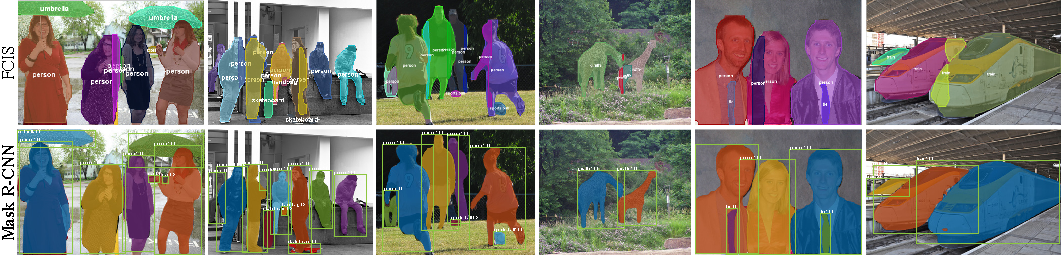
\includegraphics[width=1.0\linewidth]{figures/mask_rcnn/results_vs_fcis}
\caption{FCIS+++(上) 对比 Mask R-CNN(下, 以ResNet-101-FPN为主干). FCIS在重叠的实例中显示了系统性的错误。}
\label{fig:results_vs_fcis}
\end{figure*}

\begin{table*}[t]
% subfloat a - BackBone Architecture
\subfloat[\textbf{主干模型体系结构}: 更好的主干模型带来预期的收益:更深的网络效果更好,FPN优于C4特征,ResNeXt改进了ResNet。\label{tab:ablation:backbone}]{
\tablestyle{2.5pt}{1.05}\begin{tabular}{c|x{22}x{22}x{22}}
 \scriptsize \emph{net-depth-features} & AP & AP$_{50}$ & AP$_{75}$\\
\shline
 \scriptsize ResNet-50-C4 & 30.3 & 51.2 & 31.5\\
 \scriptsize ResNet-101-C4 & 32.7 & 54.2 & 34.3\\\hline
 \scriptsize ResNet-50-FPN & 33.6 & 55.2 & 35.3\\
 \scriptsize ResNet-101-FPN & 35.4 & 57.3 & 37.5\\
 \scriptsize ResNeXt-101-FPN & \textbf{36.7} & \textbf{59.5} & \textbf{38.9}
\end{tabular}}\hspace{1mm}
% subfloat b - Multinomial vs Independent Masks
\subfloat[\textbf{耦合的对比解耦的遮罩分支} (ResNet-50-C4): 通过每个类别的二元遮罩\emph{解耦}相比于耦合的遮罩预测有了很大提升。\label{tab:ablation:sigmoid}]{
\tablestyle{4.8pt}{1.05}\begin{tabular}{c|x{22}x{22}x{22}}
 & AP & AP$_{50}$ & AP$_{75}$\\
\shline
 \emph{softmax} & 24.8 & 44.1 & 25.1\\
 \emph{sigmoid} & \textbf{30.3} & \textbf{51.2} & \textbf{31.5}\\
\hline
 & \dt{+5.5} & \dt{+7.1} & \dt{+6.4}\\
 \multicolumn{4}{c}{~}\\
 \multicolumn{4}{c}{~}\\
\end{tabular}}\hspace{1mm}
% subfloat c - RoIAlign (ResNet-50-C4)
\subfloat[\textbf{RoIAlign} (ResNet-50-C4): 用各种RoI图层的遮罩预测结果。我们的RoIAlign层使平均精度提高了3个百分点,AP$_{75}$大约提高了5个百分点。使用适当的对齐是影响RoI层之间巨大差距的唯一因素。\label{tab:ablation:roialign}]{
\tablestyle{2.2pt}{1.05}\begin{tabular}{c|c|c|c|x{22}x{22}x{22}}
 & \scriptsize\textbf{align?} & \scriptsize bilinear? & \scriptsize agg.
 & AP & AP$_{50}$ & AP$_{75}$\\
\shline
 \emph{RoIPool}
  & & & max & 26.9 & 48.8 & 26.4\\
\hline
 \multirow{2}{*}{\emph{RoIWarp} }
  & & \checkmark & max & 27.2 & 49.2 & 27.1\\
  & & \checkmark & ave & 27.1 & 48.9 & 27.1\\
\hline
 \multirow{2}{*}{\emph{RoIAlign}}
  & \checkmark & \checkmark & max & \textbf{30.2} & \textbf{51.0} & \textbf{31.8}\\
  & \checkmark & \checkmark & ave & \textbf{30.3} & \textbf{51.2} & \textbf{31.5}
\end{tabular}}\\
% subfloat d - RoIAlign (ResNet-50-C5)
\subfloat[\textbf{RoIAlign} (ResNet-50-\textbf{C5}, \emph{stride 32}): 使用大步长特征的遮罩任务和边界框任务的平均精度。错位比步长为16的特征更严重(表\ref{tab:ablation:roialign}),导致较大的精度差距。\label{tab:ablation:roialign32}]{
\tablestyle{4pt}{1.05}\begin{tabular}{c|x{22}x{22}x{22}|x{22}x{22}x{22}}
 & AP & AP$_{50}$ & AP$_{75}$
 & AP$^\text{bb}$ & AP$^\text{bb}_{50}$ & AP$^\text{bb}_{75}$ \\[.1em]
\shline
 \emph{RoIPool} & 23.6 & 46.5 & 21.6 & 28.2 & 52.7 & 26.9\\
 \emph{RoIAlign} & \textbf{30.9} & \textbf{51.8} & \textbf{32.1} & \textbf{34.0} & \textbf{55.3} & \textbf{36.4}\\
\hline
 & \dt{+7.3} & \dt{+ 5.3} & \dt{+10.5} & \dt{+5.8} & \dt{+2.6} & \dt{+9.5}
\end{tabular}}\hspace{2mm}
% subfloat e - mask representation
\subfloat[\textbf{遮罩分支 } (ResNet-50-FPN): 全卷积网络(FCN)对比多层感知机(MLP,全连接的)用于遮罩预测。FCN改善了结果,因为它们利用了明确编码的空间布局的优势。\label{tab:ablation:maskhead}]{
\tablestyle{4pt}{1.05}\begin{tabular}{c|c|x{22}x{22}x{22}}
 & mask branch & AP & AP$_{50}$ & AP$_{75}$\\
\shline
 MLP & fc: 1024$\rightarrow$1024$\rightarrow$$80\ncdot28^2$  & 31.5 & 53.7 & 32.8\\
 MLP & fc: 1024$\rightarrow$1024$\rightarrow$1024$\rightarrow$$80\ncdot28^2$ & 31.5 & 54.0 & 32.6\\
\hline
 \textbf{FCN} &  conv: 256$\rightarrow$256$\rightarrow$256$\rightarrow$256$\rightarrow$256$\rightarrow$80
 & \textbf{33.6} & \textbf{55.2} & \textbf{35.3}
\end{tabular}}
% main caption
\caption{\textbf{对比试验}。我们在\texttt{trainval35k}上训练,在\texttt{minival}上测试。除非特别说明,以上都是\emph{遮罩}平均精度指标。}
\label{tab:ablations}
\end{table*}

\xjtuappendixsubsection{控制变量对比试验}\label{sec:ablations}

我们对Mask R-CNN进行了一系列的控制变量对比实验分析。结果显示在表\ref{tab:ablations}中并在下面详细讨论。

\paragraph{体系结构:} 表\ref{tab:ablation:backbone}展示了Mask R-CNN在不同的主干模型下的结果。Mask R-CNN受益于更深的网络(50层对比101层)和先进的设计,包括FPN和ResNeXt。 我们注意到\emph{不是}所有框架都会自动从更深或更高级的网络中受益。

\paragraph{耦合的和解耦的遮罩分支:} Mask R-CNN将遮罩预测和类别预测\emph{解耦}:现有的边界框分支已经可以预测类别标签,因此我们为每个类别生成一个遮罩,而不会造成类别的冲突(由于每个像素的\emph{sigmoid}函数和\emph{二元}损失)。 在表\ref{tab:ablation:sigmoid}中,我们将其与对每个像素进行\emph{softmax}激活和多项损失(如FCN中常用的)进行比较。这种替代方案将遮罩和类别预测任务相\emph{耦合},并导致遮罩平均精度下降了5.5个百分点。 这表明,一旦实例被整体分类(通过边界框分支),就足够预测二元遮罩了,而不用考虑类别,这使得模型更易于训练。

\paragraph{类别已知和类别不可知的遮罩预测:} 我们默认的实例化模型是在类别已知的情况下进行遮罩预测的。例如对于每一个类别,都会预测一个$m\times m$的遮罩。有趣的是,在类别不可知的情况下(例如无论类别如何,只输出一个$m\times m$的遮罩),Mask R-CNN几乎同样有效:其取得了29.7的遮罩均值精度,相比于类别已知模型30.3的均值精度,它们都是以ResNet-50-C4为主干模型。这进一步突出了我们的方法中的分工,这在很大程度上使得分类任务和分割任务解耦。

\begin{table*}[t]
\tablestyle{3.5pt}{1.1}
\begin{tabular}{l|l|x{22}x{22}x{22}|x{22}x{22}x{22}}
 & backbone
 & AP$^\text{bb}$ & AP$^\text{bb}_{50}$ & AP$^\text{bb}_{75}$
 & AP$^\text{bb}_S$ & AP$^\text{bb}_M$ &  AP$^\text{bb}_L$\\ [.1em]
\shline
 Faster R-CNN+++  & ResNet-101-C4
  & 34.9 & 55.7 & 37.4 & 15.6 & 38.7 & 50.9\\
 Faster R-CNN w FPN  & ResNet-101-FPN
  & 36.2 & 59.1 & 39.0 & 18.2 & 39.0 & 48.2\\
 Faster R-CNN by G-RMI  & Inception-ResNet-v2
  & 34.7 & 55.5 & 36.7 & 13.5 & 38.1 & 52.0\\
 Faster R-CNN w TDM  & Inception-ResNet-v2-TDM
  & 36.8 & 57.7 & 39.2 & 16.2 & 39.8 & \textbf{52.1}\\
\hline
  Faster R-CNN, RoIAlign & ResNet-101-FPN
  & 37.3 & 59.6 & 40.3 & 19.8 & 40.2 & 48.8\\
 \textbf{Mask R-CNN} & ResNet-101-FPN
  & 38.2 & 60.3 & 41.7 & 20.1 & 41.1 & 50.2\\
 \textbf{Mask R-CNN} & ResNeXt-101-FPN
  & \textbf{39.8} & \textbf{62.3} & \textbf{43.4} & \textbf{22.1} & \textbf{43.2} & {51.2}
\end{tabular}
\caption{\textbf{目标检测} \emph{单一模型} 的结果 (边界框均值精度), 对比该领域最先进的方法,在\texttt{test-dev}测试集上. 使用ResNet-101-FPN作为主干模型的Mask R-CNN的表现超过了所有先前该领最先进的模型的基础变种(在这个任务中,遮罩预测输出会被直接忽略)。Mask R-CNN相对于Faster R-CNN的提升主要来自于使用了RoIAlign(+1.1 $AP^\text{bb}$)、多任务训练(+0.9 AP$^\text{bb}$)以及ResNeXt-101(+1.6 AP$^\text{bb}$)。}
\label{tab:final_bbox}
\end{table*}

\paragraph{RoIAlign:} 我们提出的\emph{RoIAlign}层的性能评估如表\ref{tab:ablation:roialign}所示。对于这个实验,我们使用了步长为16的ResNet-50-C4作为主干模型。RoIAlign相比于RoIPool在均值精度上提升了3个百分点,其中大部分收益来自高IoU(例如AP$_{75}$)。RoIAlign对最大池化或平均池化不敏感;我们在本文的其余部分均使用平均池化。

此外,我们与在MNC中提出的\emph{RoIWarp}做了比较,其同样采用了双线性采样。正如在\S\ref{sec:maskR-CNN}所讨论的,RoIWarp依然量化RoI,使得与输入不对齐。从表\ref{tab:ablation:roialign}可以看出,RoIWarp 的表现与RoIPool相当,但比RoIAlign差很多。这突出表明正确的对齐是很关键的。

我们还对以\emph{ResNet-50-C5}作为主干模型的RoIAlign进行了评估,该主干模型以更大的32像素作为步长。我们使用与图\ref{fig:head}(右)中相同的前部,因为res5与此不兼容。从表\ref{tab:ablation:roialign32}可看出,RoIAlign在均值精度上提升了7.3个百分点,在遮罩AP$_{75}$提升了10.5个百分点(\emph{50\%的相对提升})。更进一步地,我们注意到对于RoIAlign,使用\emph{stride-32} C5特征(30.9 AP)比使用stride-16 C4特征(30.3 AP, 表\ref{tab:ablation:roialign})更加精准。RoIAlignn 在很大程度上解决了使用大步长特征进行检测和分割的长期挑战。

最后,与FPN一起使用时,RoIAlign在遮罩均值精度上能得到1.5个百分点的提升,在边界框均值精度上得到0.1),RoIAlign即使使用FPN(表\ref{tab:roialign_keypoint})也显示出较大的提升。

\paragraph{遮罩预测分支:} 分割是像素到像素的任务,我们通过使用FCN来利用遮罩的空间布局。在表\ref{tab:ablation:maskhead}中,我们比较了多层感知机(MLP)和使用了ResNet-50-FPN作为主干模型的FCN。使用FCN相对于MLP在遮罩均值精度上提升了2.1个百分点。我们注意到,我们选择这个骨干,以便FCN前部的卷积层没有预先训练,以公平地与MLP比较。

\xjtuappendixsubsection{边界框检测结果}

我们将Mask R-CNN与表\ref{tab:final_bbox}中的最新 COCO \emph{边界框}目标检测进行了比较。对于这个结果,即使完整的Mask R-CNN模型被训练,只有分类和边界框输出用于预测(遮罩输出被忽略)。 使用ResNet-101-FPN的Mask R-CNN优于所有先前最先进的模型的基础变种,包括G-RMI的单一模型,其为COCO 2016目标检测挑战赛的获胜者。通过使用ResNeXt-101-FPN,Mask R-CNN 进一步提高了结果,与之前使用 Inception-ResNet-v2-TDM的最佳单一模型相比,边界框均值精度提升了3.0个百分点。

作为进一步的比较,我们训练了一个\emph{没有}遮罩预测分支的Mask R-CNN版本,在表\ref{tab:final_bbox}中记为``Faster R-CNN, RoIAlign''。由于RoIAlign的原因,该模型的表现要好于模型Faster R-CNN。另一方面,该模型比Mask R-CNN低0.9个百分点的均值精度。因此Mask R-CNN在边界框检测上的这种优势是由于多任务训练的带来好处。

最后,我们注意到Mask R-CNN在它的遮罩和边界框均值精度上有一个小的差距:例如,37.1(遮罩,表\ref{tab:final_mask})和39.8(边界框,表\ref{tab:final_bbox})之间的2.7个百分点。这表明我们的方法在很大程度上缩小了目标检测与更具挑战性的实例分割任务之间的差距。

\xjtuappendixsubsection{时间性能}

\paragraph{预测:} 我们在Faster R-CNN的4步训练之后训练一个在RPN和Mask R-CNN阶段共享特征的ResNet-101-FPN模型。在Nvidia Tesla M40 GPU上,该模型以每张图片195毫秒的速度运行(加上15m毫秒的CPU时间,将输出调整为原始分辨率),并实现了在统计意义上的与非共享模式相同的遮罩均值精度。我们还表示使用ResNet-101-C4的变体大约需要耗时400毫秒,因为其拥有一个计算任务更重的前部(图\ref{fig:head}),因此我们不推荐在实践中使用 C4 变体。

虽然Mask R-CNN速度很快,但我们注意到我们的设计并未针对速度进行优化,并且可以进一步改进以实现更好的速度和精确度折衷,例如,通过改变图像尺寸和候选框数量,不过这超出了本文的范围。

\paragraph{训练:} Mask R-CNN 的训练也很快。 在COCO\texttt{trainval35k}数据集上使用ResNet-50-FPN进行训练需要32小时的时间。我们同步使用8个GPU(每个最小批量有16张图像,耗时0.72秒)。若是训练ResNet-101-FPN则需要44个小时。 实际上,在\texttt{train}数据集上训练时,可以在\emph{一天之内}完成快速原型。我们希望这种快速训练能够消除该领域的一个主要障碍,并鼓励更多的人对这个具有挑战性的话题进行研究。

\begin{figure*}[t]
\centering
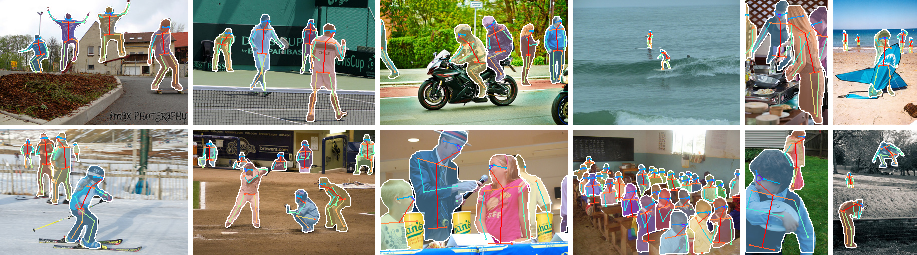
\includegraphics[width=1.0\linewidth]{figures/mask_rcnn/results_keypoints}
\caption{在COCO \texttt{test}数据集上使用Mask R-CNN(ResNet-50-FPN)进行关键点检测,包括从相同模型中预测出的人物分割遮罩。此模型的关键点均值精度为63.1,速度为每秒5张图片。}
\label{fig:results_keypoints}
\end{figure*}

\xjtuappendixsection{Mask R-CNN用于人体姿势估计}\label{sec:keypoints}

我们的框架可以很容易地扩展到人体姿态估计。我们将一个关键点的位置建模为二元遮罩,并采用Mask R-CNN来预测$K$个遮罩,每个遮罩用于表示$K$个关键点类型(例如,左肩,右肘)中的一个。这项任务有助于展示Mask R-CNN的灵活性。

我们注意到,我们的系统利用了人类姿态的\emph{最小}领域知识,因为实验主要是为了展示Mask R-CNN框架的通用性。我们期望领域知识(例如建模结构)会与我们简单的方法相辅相成。

\paragraph{实现细节:} 我们在将模型应用到对关键点预测时对分割系统进行了细微的修改。对于实例的$K$个关键点中的每个关键点,训练目标是二元$m\times m$的二进制遮罩,其中只有\emph{一个}像素被标记为前景。在训练期间,对于每个可见的真实关键点,我们将$m^2$路通过softmax输出(它鼓励单个点被检测到),并使用交叉熵损失进行最小化优化。我们注意到,与实例分割一样,$K$个关键点仍然是独立处理的。

我们采用了一个ResNet-FPN变体,其关键点前部结构与图\ref{fig:head}(右)相似。关键点前部由8个$3\times3$的、包含512个卷积核的卷积层组成,后面是去卷积层和2倍双线性放大,产生$56\times56$的输出分辨率。我们发现相对较高的分辨率输出(与遮罩分支相比)是关键点级别的定位精度所必需的。

模型在包含标注好关键点的COCO \texttt{trainval35k} 所有图像上进行训练。由于该训练集较小,为了减少过拟合,我们使用从 [640,800] 像素随机采样的图像进行训练。预测是在800像素的单一尺度上进行的。我们训练9万次迭代,从0.02的学习率开始,在6万和8万迭代时将其减少为当前的$1/10$。我们使用边界框NMS,阈值为0.5。其他细节与\S\ref{sec:impl}中的相同。

\begin{table}[t]
\tablestyle{1.8pt}{1.2}
\begin{tabular}{l|x{22}x{22}x{22}|x{22}x{22}}
 & AP$^\text{kp}$ & AP$^\text{kp}_{50}$ & AP$^\text{kp}_{75}$
 & AP$^\text{kp}_M$ &  AP$^\text{kp}_L$\\ [.1em]
\shline
CMU-Pose+++  & 61.8 & 84.9 & 67.5 & 57.1 & 68.2 \\
G-RMI $^\dagger$ & 62.4 & 84.0 & 68.5 & \textbf{59.1} & 68.1 \\
\hline
 \textbf{Mask R-CNN}, \footnotesize keypoint-only & 62.7 & 87.0 & 68.4 & 57.4 & 71.1 \\
 \textbf{Mask R-CNN}, \footnotesize keypoint \& mask & \textbf{63.1} & \textbf{87.3} & \textbf{68.7} & {57.8} & \textbf{71.4} \\
\end{tabular}
\caption{\textbf{关键点检测} 在COCO \texttt{test-dev}数据集上的均值精度. 我们的模型是一个单一模型(ResNet-50-FPN),运行的速度为每秒5张图片。CMU-Pose+++ is 2016挑战的获胜者,其使用了多尺度测试,使用CPM进行后续处理,并且使用目标检测器进行过滤。我们的方法相比它提升了大约5个百分点(在个人通讯中声明)。$^\dagger$:G-RMI在COCO数据集\emph{以及}MPII数据集(2.5万张图片)上训练,使用两个模型(Inception-ResNet-v2用于边界框检测,ResNet-101用于关键点检测)。}
\label{tab:final_keypoint}
\end{table}

\paragraph{主要结果以及控制变量分析:}我们评估人体关键点的均值精度AP(AP$^\text{kp}$)并在实验中ResNet-50-FPN作为主干;附录中将研究更多主干模型。表\ref{tab:final_keypoint}显示我们的结果(62.7 AP$^\text{kp}$)比使用多级处理流水线的 COCO 2016关键点检测获胜者高0.9个百分点(请参阅表\ref{tab:final_keypoint}的标题)。我们的方法相当简单快捷。

\begin{table}[t]
\begin{minipage}{0.55\textwidth}
  \tablestyle{7pt}{1.1}
  \begin{tabular}{l|x{22}x{22}x{22}}
  & AP$^\text{bb}_\text{\emph{person}}$ & AP$^\text{mask}_\text{\emph{person}}$
  & AP$^\text{kp}$ \\ [.1em]
  \shline
  Faster R-CNN & 52.5 & - & - \\
  Mask R-CNN, mask-only & \textbf{53.6} & \textbf{45.8} & - \\
  Mask R-CNN, keypoint-only & 50.7 & - & 64.2 \\
  Mask R-CNN, keypoint \& mask & 52.0 & 45.1 & \textbf{64.7} \\
  \end{tabular}
  \caption{对于\emph{人类}领域的边界框、遮罩以及关键点的\textbf{多任务学习},在\texttt{minival}数据集上的评估结果。所有的对比模型都使用相同的数据进行公平比较。主干模型是ResNet-50-FPN。在\texttt{minival}数据集上的均值精度为64.2和64.7模型在\texttt{test-dev}数据集上的均值精度分别为62.7和63.1(见表\ref{tab:final_keypoint})。}
  \label{tab:multitask_keypoint}
\end{minipage}\hspace{3mm}
\begin{minipage}{0.4\textwidth}
  \tablestyle{2pt}{1.1}
  \begin{tabular}{l|x{22}x{22}x{22}|x{22}x{22}}
   & AP$^\text{kp}$ & AP$^\text{kp}_{50}$ & AP$^\text{kp}_{75}$
   & AP$^\text{kp}_M$ &  AP$^\text{kp}_L$\\ [.1em]
  \shline
   \emph{RoIPool} & 59.8 & 86.2 & 66.7 & 55.1 & 67.4 \\
   \emph{RoIAlign}~~~~ & \textbf{64.2} & \textbf{86.6} & \textbf{69.7} & \textbf{58.7} & \textbf{73.0} \\
  \end{tabular}
  \caption{\textbf{RoIAlign 对比 RoIPool}用于关键点检测,在\texttt{minival}数据集上,主干模型为ResNet-50-FPN。}
  \label{tab:roialign_keypoint}
\end{minipage}
\end{table}

更重要的是,我们实现了\emph{一个可以同时预测边界框,遮罩和关键点的统一模型},而且可以以5 fps的速度运行。添加遮罩分支(针对人员类别)在\texttt{test-dev}数据集上将AP$^\text{kp}$提升了为63.1(表\ref{tab:final_keypoint})。表\ref{tab:multitask_keypoint}中更详细地讨论了\texttt{minival}上的多任务学习。将\emph{遮罩}分支添加到只有边界框的模型中(例如Faster R-CNN)或只有关键点的版本中可以持续改进这些任务。但是,添加关键点分支会略微减少边界框或遮罩任务的均值精度,这表明虽然关键点检测可从多任务训练中受益,但它不会帮助其它任务。不过,共同学习所有三项任务可以使统一系统同时有效地预测所有输出(图\ref{fig:results_keypoints})。

我们还调研了\emph{RoIAlign}对关键点检测(表\ref{tab:roialign_keypoint})的影响。尽管此ResNet-50-FPN主干具有更好的步长(例如最好的水平上有4个像素),但RoIAlign仍然比RoIPool有显着的提升,并将AP$^\text{kp}$提高了4.4个百分点。这是因为关键点检测对定位精度更敏感。这再次表明,对齐对像素级定位至关重要,包括遮罩和关键点。

鉴于Mask R-CNN在提取目标边界框、遮罩和关键点的有效性,我们预计它将成为其他实例级任务的有效框架。

\begin{table*}[t]
\tablestyle{4pt}{1.05}
\begin{tabular}{l|l|x{32}|x{22}x{22}|x{22}x{22}x{22}x{22}x{22}x{22}x{22}x{22}}
 & \multicolumn{1}{c|}{training data} & AP [\texttt{val}] & AP & AP$_{50}$
 & person & rider & car & truck & bus & train & mcycle & bicycle\\[.1em]
\shline
 InstanceCut  & \texttt{fine} + \texttt{coarse}
  & 15.8 & 13.0 & 27.9 & 10.0 & 8.0 & 23.7 & 14.0 & 19.5 & 15.2 & 9.3 & 4.7 \\
 DWT  & \texttt{fine}
  & 19.8 & 15.6 & 30.0 & 15.1 & 11.7 & 32.9 & 17.1 & 20.4 & 15.0 & 7.9 & 4.9 \\
 SAIS  & \texttt{fine}
  & - & 17.4 & 36.7 & 14.6 & 12.9 & 35.7 & 16.0 & 23.2 & 19.0 & 10.3 & 7.8 \\
 DIN  & \texttt{fine} + \texttt{coarse}
  & - & 20.0 & 38.8 & 16.5 & 16.7 & 25.7 & 20.6 & 30.0 & 23.4 & 17.1 & 10.1 \\
 SGN  & \texttt{fine} + \texttt{coarse} & 29.2 & 25.0 & 44.9 & 21.8 &	20.1 &	39.4 &	24.8 &	33.2 &	30.8 &	17.7 &	12.4 \\
\hline
 Mask R-CNN & \texttt{fine}
  & 31.5 & 26.2 & 49.9 & 30.5 & 23.7 & 46.9 & 22.8 & 32.2 & 18.6 & 19.1 & 16.0 \\
 Mask R-CNN & \texttt{fine} + COCO
  & \textbf{36.4} & \textbf{32.0} & \textbf{58.1} & \textbf{34.8} & \textbf{27.0} & \textbf{49.1} & \textbf{30.1} & \textbf{40.9} & \textbf{30.9} & \textbf{24.1} & \textbf{18.7} \\
\end{tabular}
\caption{在Cityscapes \texttt{val} (`AP [\texttt{val}]' 列) and \texttt{test} (其它列)数据集上的结果。我们的方法使用ResNet-50-FPN作为主干。}
\label{tab:cityscapes}
\end{table*}


%===============================================================================


\xjtuappendixchapter{外文文献原文}

\begin{center}
    \sihao\textbf{Mask R-CNN}
\end{center}

\textbf{ABSTRACT}: We present a conceptually simple, flexible, and general framework for object instance segmentation. Our approach efficiently detects objects in an image while simultaneously generating a high-quality segmentation mask for each instance. The method, called Mask R-CNN, extends Faster R-CNN by adding a branch for predicting an object mask in \emph{parallel} with the existing branch for bounding box recognition. Mask R-CNN is simple to train and adds only a small overhead to Faster R-CNN, running at 5 fps. Moreover, Mask R-CNN is easy to generalize to other tasks, e.g., allowing us to estimate human poses in the same framework. We show top results in all three tracks of the COCO suite of challenges, including instance segmentation, bounding-box object detection, and person keypoint detection. Without bells and whistles, Mask R-CNN outperforms all existing, single-model entries on every task, including the COCO 2016 challenge winners. We hope our simple and effective approach will serve as a solid baseline and help ease future research in instance-level recognition. Code has been made available at: \url{https://github.com/facebookresearch/Detectron}.

\xjtuappendixsection{Introduction}

The vision community has rapidly improved object detection and semantic segmentation results over a short period of time. In large part, these advances have been driven by powerful baseline systems, such as the Fast/Faster R-CNN and Fully Convolutional Network (FCN) frameworks for object detection and semantic segmentation, respectively. These methods are conceptually intuitive and offer flexibility and robustness, together with fast training and inference time. Our goal in this work is to develop a comparably enabling framework for \emph{instance segmentation}.

\begin{figure}
\begin{minipage}{0.35\textwidth}
  \centering
  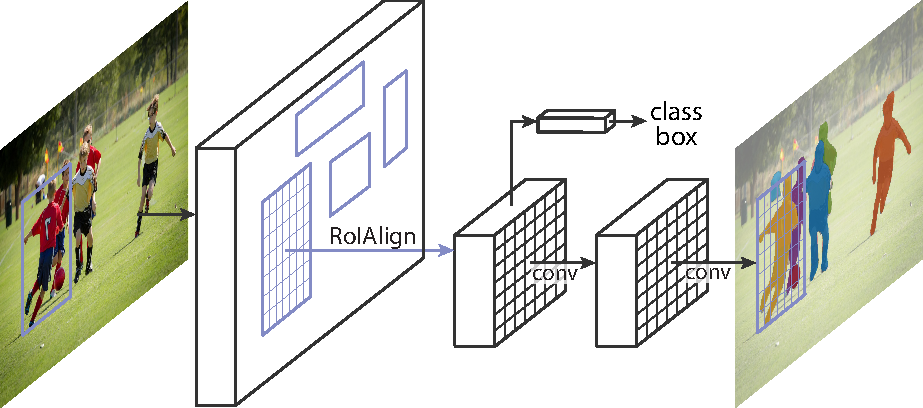
\includegraphics[width=1\linewidth]{figures/mask_rcnn/teaser}\vspace{2mm}
  \caption{The \textbf{Mask\hspace{0.1297em}R-CNN} framework for instance segmentation.}
\label{fig:teaser}
\end{minipage}\hspace{1.5em}
\begin{minipage}{0.6\textwidth}
  \begin{minipage}{0.365\linewidth}
  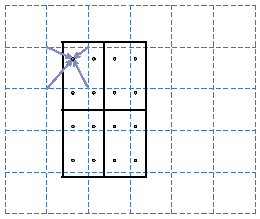
\includegraphics[width=\textwidth,trim={0 0 7.5mm 0},clip]{figures/mask_rcnn/roialign}
  \end{minipage}\hspace{0.5em}
  \begin{minipage}{0.605\linewidth}
  \caption{\footnotesize \textbf{RoIAlign:} The dashed grid represents a feature map, the solid lines an RoI (with 2$\times$2 bins in this example), and the dots the 4 sampling points in each bin. RoIAlign computes the value of each sampling point by bilinear interpolation from the nearby grid points on the feature map. No quantization is performed on any coordinates involved in the RoI, its bins, or the sampling points.}
  \label{fig:roialign}
  \end{minipage}
\end{minipage}
\end{figure}

Instance segmentation is challenging because it requires the correct detection of all objects in an image while also precisely segmenting each instance. It therefore combines elements from the classical computer vision tasks of \emph{object detection}, where the goal is to classify individual objects and localize each using a bounding box, and \emph{semantic segmentation}, where the goal is to classify each pixel into a fixed set of categories without differentiating object instances.\footnote{Following common terminology, we use \emph{object detection} to denote detection via \emph{bounding boxes}, not masks, and \emph{semantic segmentation} to denote per-pixel classification without differentiating instances. Yet we note that \emph{instance segmentation} is both semantic and a form of detection.}~Given this, one might expect a complex method is required to achieve good results. However, we show that a surprisingly simple, flexible, and fast system can surpass prior state-of-the-art instance segmentation results.

Our method, called \emph{Mask R-CNN}, extends Faster R-CNN by adding a branch for predicting segmentation masks on each Region of Interest (RoI), in \emph{parallel} with the existing branch for classification and bounding box regression (Figure~\ref{fig:teaser}). The mask branch is a small FCN applied to each RoI, predicting a segmentation mask in a pixel-to-pixel manner. Mask R-CNN is simple to implement and train given the Faster R-CNN framework, which facilitates a wide range of flexible architecture designs. Additionally, the mask branch only adds a small computational overhead, enabling a fast system and rapid experimentation.

In principle Mask R-CNN is an intuitive extension of Faster R-CNN, yet constructing the mask branch properly is critical for good results. Most importantly, Faster R-CNN was not designed for pixel-to-pixel alignment between network inputs and outputs. This is most evident in how \emph{RoIPool}, the \emph{de facto} core operation for attending to instances, performs coarse spatial quantization for feature extraction. To fix the misalignment, we propose a simple, quantization-free layer, called \emph{RoIAlign}, that faithfully preserves exact spatial locations. Despite being a seemingly minor change, RoIAlign has a large impact: it improves mask accuracy by relative 10\% to 50\%, showing bigger gains under stricter localization metrics. Second, we found it essential to \emph{decouple} mask and class prediction: we predict a binary mask for each class independently, without competition among classes, and rely on the network's RoI classification branch to predict the category. In contrast, FCNs usually perform per-pixel multi-class categorization, which couples segmentation and classification, and based on our experiments works poorly for instance segmentation.

Without bells and whistles, Mask R-CNN surpasses all previous state-of-the-art single-model results on the COCO instance segmentation task, including the heavily-engineered entries from the 2016 competition winner. As a by-product, our method also excels on the COCO object detection task. In ablation experiments, we evaluate multiple basic instantiations, which allows us to demonstrate its robustness and analyze the effects of core factors.

Our models can run at about 200ms per frame on a GPU, and training on COCO takes one to two days on a single 8-GPU machine. We believe the fast train and test speeds, together with the framework's flexibility and accuracy, will benefit and ease future research on instance segmentation.

Finally, we showcase the generality of our framework via the task of human pose estimation on the COCO keypoint dataset. By viewing each keypoint as a one-hot binary mask, with minimal modification Mask R-CNN can be applied to detect instance-specific poses. Mask R-CNN surpasses the winner of the 2016 COCO keypoint competition, and at the same time runs at 5 fps. Mask R-CNN, therefore, can be seen more broadly as a flexible framework for \emph{instance-level recognition} and can be readily extended to more complex tasks.

We have released code to facilitate future research.

\xjtuappendixsection{Related Work}

\paragraph{R-CNN:} The Region-based CNN (R-CNN) approach to bounding-box object detection is to attend to a manageable number of candidate object regions and evaluate convolutional networks  independently on each RoI. R-CNN was extended to allow attending to RoIs on feature maps using RoIPool, leading to fast speed and better accuracy. Faster R-CNN advanced this stream by learning the attention mechanism with a Region Proposal Network (RPN). Faster R-CNN is flexible and robust to many follow-up improvements (e.g.,), and is the current leading framework in several benchmarks.

\paragraph{Instance Segmentation:} Driven by the effectiveness of R-CNN, many approaches to instance segmentation are based on \emph{segment proposals}. Earlier methods resorted to bottom-up segments. DeepMask and following works learn to propose segment candidates, which are then classified by Fast R-CNN. In these methods, segmentation \emph{precedes} recognition, which is slow and less accurate. Likewise, Dai et al. proposed a complex multiple-stage cascade that predicts segment proposals from bounding-box proposals, followed by classification. Instead, our method is based on \emph{parallel} prediction of masks and class labels, which is simpler and more flexible.

Most recently, Li et al. combined the segment proposal system in and object detection system in for ``fully convolutional instance segmentation'' (FCIS). The common idea in is to predict a set of position-sensitive output channels fully convolutionally. These channels simultaneously address object classes, boxes, and masks, making the system fast. But FCIS exhibits systematic errors on overlapping instances and creates spurious edges (Figure~\ref{fig:results_vs_fcis}), showing that it is challenged by the fundamental difficulties of segmenting instances.

Another family of solutions to instance segmentation are driven by the success of semantic segmentation. Starting from per-pixel classification results (e.g., FCN outputs), these methods attempt to cut the pixels of the same category into different instances. In contrast to the \emph{segmentation-first} strategy of these methods, Mask R-CNN is based on an \emph{instance-first} strategy. We expect a deeper incorporation of both strategies will be studied in the future.

\xjtuappendixsection{Mask R-CNN}\label{sec:maskrcnn}

Mask R-CNN is conceptually simple: Faster R-CNN has two outputs for each candidate object, a class label and a bounding-box offset; to this we add a third branch that outputs the object mask. Mask R-CNN is thus a natural and intuitive idea. But the additional mask output is distinct from the class and box outputs, requiring extraction of much \emph{finer} spatial layout of an object. Next, we introduce the key elements of Mask R-CNN, including pixel-to-pixel alignment, which is the main missing piece of Fast/Faster R-CNN.

\paragraph{Faster R-CNN:} We begin by briefly reviewing the Faster R-CNN detector. Faster R-CNN consists of two stages. The first stage, called a Region Proposal Network (RPN), proposes candidate object bounding boxes. The second stage, which is in essence Fast R-CNN, extracts features using RoIPool from each candidate box and performs classification and bounding-box regression. The features used by both stages can be shared for faster inference. We refer readers to for latest, comprehensive comparisons between Faster R-CNN and other frameworks.

\paragraph{Mask R-CNN:} Mask R-CNN adopts the same two-stage procedure, with an identical first stage (which is RPN). In the second stage, \emph{in parallel} to predicting the class and box offset, Mask R-CNN also outputs a binary mask for each RoI. This is in contrast to most recent systems, where classification \emph{depends} on mask predictions (e.g.). Our approach follows the spirit of Fast R-CNN that applies bounding-box classification and regression in \emph{parallel} (which turned out to largely simplify the multi-stage pipeline of original R-CNN).

Formally, during training, we define a multi-task loss on each sampled RoI as $L = L_{cls} + L_{box} + L_{mask}$. The classification loss $L_{cls}$ and bounding-box loss $L_{box}$ are identical as those defined in. The mask branch has a $Km^2$-dimensional output for each RoI, which encodes $K$ binary masks of resolution $m \times m$, one for each of the $K$ classes. To this we apply a per-pixel sigmoid, and define $L_{mask}$ as the average binary cross-entropy loss. For an RoI associated with ground-truth class $k$, $L_{mask}$ is only defined on the $k$-th mask (other mask outputs do not contribute to the loss).

Our definition of $L_{mask}$ allows the network to generate masks for every class without competition among classes; we rely on the dedicated classification branch to predict the class label used to select the output mask. This \emph{decouples} mask and class prediction. This is different from common practice when applying FCNs to semantic segmentation, which typically uses a per-pixel \emph{softmax} and a \emph{multinomial} cross-entropy loss. In that case, masks across classes compete; in our case, with a per-pixel \emph{sigmoid} and a \emph{binary} loss, they do not. We show by experiments that this formulation is key for good instance segmentation results.

\paragraph{Mask Representation:} A mask encodes an input object's \emph{spatial} layout. Thus, unlike class labels or box offsets that are inevitably collapsed into short output vectors by fully-connected (\emph{fc}) layers, extracting the spatial structure of masks can be addressed naturally by the pixel-to-pixel correspondence provided by convolutions.

Specifically, we predict an $m \times m$ mask from each RoI using an FCN. This allows each layer in the mask branch to maintain the explicit $m \times m$ object spatial layout without collapsing it into a vector representation that lacks spatial dimensions. Unlike previous methods that resort to \emph{fc} layers for mask prediction, our fully convolutional representation requires fewer parameters, and is more accurate as demonstrated by experiments.

This pixel-to-pixel behavior requires our RoI features, which themselves are small feature maps, to be well aligned to faithfully preserve the explicit per-pixel spatial correspondence. This motivated us to develop the following \emph{RoIAlign} layer that plays a key role in mask prediction.

\paragraph{RoIAlign:} RoIPool is a standard operation for extracting a small feature map (e.g., 7$\times$7) from each RoI. RoIPool first \emph{quantizes} a floating-number RoI to the discrete granularity of the feature map, this quantized RoI is then subdivided into spatial bins which are themselves quantized, and finally feature values covered by each bin are aggregated (usually by max pooling). Quantization is performed, e.g., on a continuous coordinate $x$ by computing $[x/16]$, where 16 is a feature map stride and $[\cdot]$ is rounding; likewise, quantization is performed when dividing into bins (e.g., 7$\times$7). These quantizations introduce misalignments between the RoI and the extracted features. While this may not impact classification, which is robust to small translations, it has a large negative effect on predicting pixel-accurate masks.

To address this, we propose an \emph{RoIAlign} layer that removes the harsh quantization of RoIPool, properly \emph{aligning} the extracted features with the input. Our proposed change is simple: we avoid any quantization of the RoI boundaries or bins (i.e., we use $x/16$ instead of $[x/16]$). We use bilinear interpolation to compute the exact values of the input features at four regularly sampled locations in each RoI bin, and aggregate the result (using max or average), see Figure~\ref{fig:roialign} for details. We note that the results are not sensitive to the exact sampling locations, or how many points are sampled, \emph{as long as} no quantization is performed.

RoIAlign leads to large improvements as we show in \S\ref{sec:ablations}. We also compare to the RoIWarp operation proposed in.
Unlike RoIAlign, RoIWarp overlooked the alignment issue and was implemented in as quantizing RoI just like RoIPool. So even though RoIWarp also adopts bilinear resampling motivated by, it performs on par with RoIPool as shown by experiments (more details in Table~\ref{tab:ablation:roialign}), demonstrating the crucial role of alignment.

\paragraph{Network Architecture:} To demonstrate the generality of our approach, we instantiate Mask R-CNN with multiple architectures. For clarity, we differentiate between: (i) the convolutional \emph{backbone} architecture used for feature extraction over an entire image, and (ii) the network \emph{head} for bounding-box recognition (classification and regression) and mask prediction that is applied separately to each RoI.

We denote the \emph{backbone} architecture using the nomenclature \emph{network-depth-features}. We evaluate ResNet and ResNeXt networks of depth 50 or 101 layers. The original implementation of Faster R-CNN with ResNets extracted features from the final convolutional layer of the 4-th stage, which we call C4. This backbone with ResNet-50, for example, is denoted by ResNet-50-C4. This is a common choice used in.

We also explore another more effective backbone recently proposed by Lin et al., called a Feature Pyramid Network (FPN). FPN uses a top-down architecture with lateral connections to build an in-network feature pyramid from a single-scale input. Faster R-CNN with an FPN backbone extracts RoI features from different levels of the feature pyramid according to their scale, but otherwise the rest of the approach is similar to vanilla ResNet. Using a ResNet-FPN backbone for feature extraction with Mask R-CNN gives excellent gains in both accuracy and speed. For further details on FPN, we refer readers to.

For the network \emph{head} we closely follow architectures presented in previous work to which we add a fully convolutional mask prediction branch. Specifically, we extend the Faster R-CNN box heads from the ResNet and FPN papers. Details are shown in Figure~\ref{fig:head}. The head on the ResNet-C4 backbone includes the 5-th stage of ResNet (namely, the 9-layer `res5'), which is compute-intensive. For FPN, the backbone already includes res5 and thus allows for a more efficient head that uses fewer filters.

We note that our mask branches have a straightforward structure. More complex designs have the potential to improve performance but are not the focus of this work.

\begin{figure}[t]
\centering
\begin{overpic}[width=1.0\linewidth]{figures/mask_rcnn/head}
  \put(33,29){Faster R-CNN}
  \put(33,26){w/ ResNet }
  \put(84,29){Faster R-CNN}
  \put(84,26){w/ FPN }
\end{overpic}
\caption{\textbf{Head Architecture}: We extend two existing Faster R-CNN heads. Left/Right panels show the heads for the ResNet C4 and FPN backbones, from and, respectively, to which a mask branch is added.
Numbers denote spatial resolution and channels.
Arrows denote either conv, deconv, or \emph{fc} layers as can be inferred from context (conv preserves spatial dimension while deconv increases it).
All convs are 3$\x$3, except the output conv which is 1$\x$1, deconvs are 2$\x$2 with stride 2, and we use ReLU in hidden layers. \emph{Left}: `res5' denotes ResNet's fifth stage, which for simplicity we altered so that the first conv operates on a 7$\x$7 RoI with stride 1 (instead of 14$\x$14 / stride 2 as in). \emph{Right}: `$\x$4' denotes a stack of four consecutive convs.}
\label{fig:head}
\end{figure}

\xjtuappendixsubsection{Implementation Details}\label{sec:impl}

We set hyper-parameters following existing Fast/Faster R-CNN work. Although these decisions were made for object detection in original papers, we found our instance segmentation system is robust to them.

\paragraph{Training:} As in Fast R-CNN, an RoI is considered positive if it has IoU with a ground-truth box of at least 0.5 and negative otherwise. The mask loss $L_{mask}$ is defined only on positive RoIs. The mask target is the intersection between an RoI and its associated ground-truth mask.

\begin{figure*}[t]
\centering
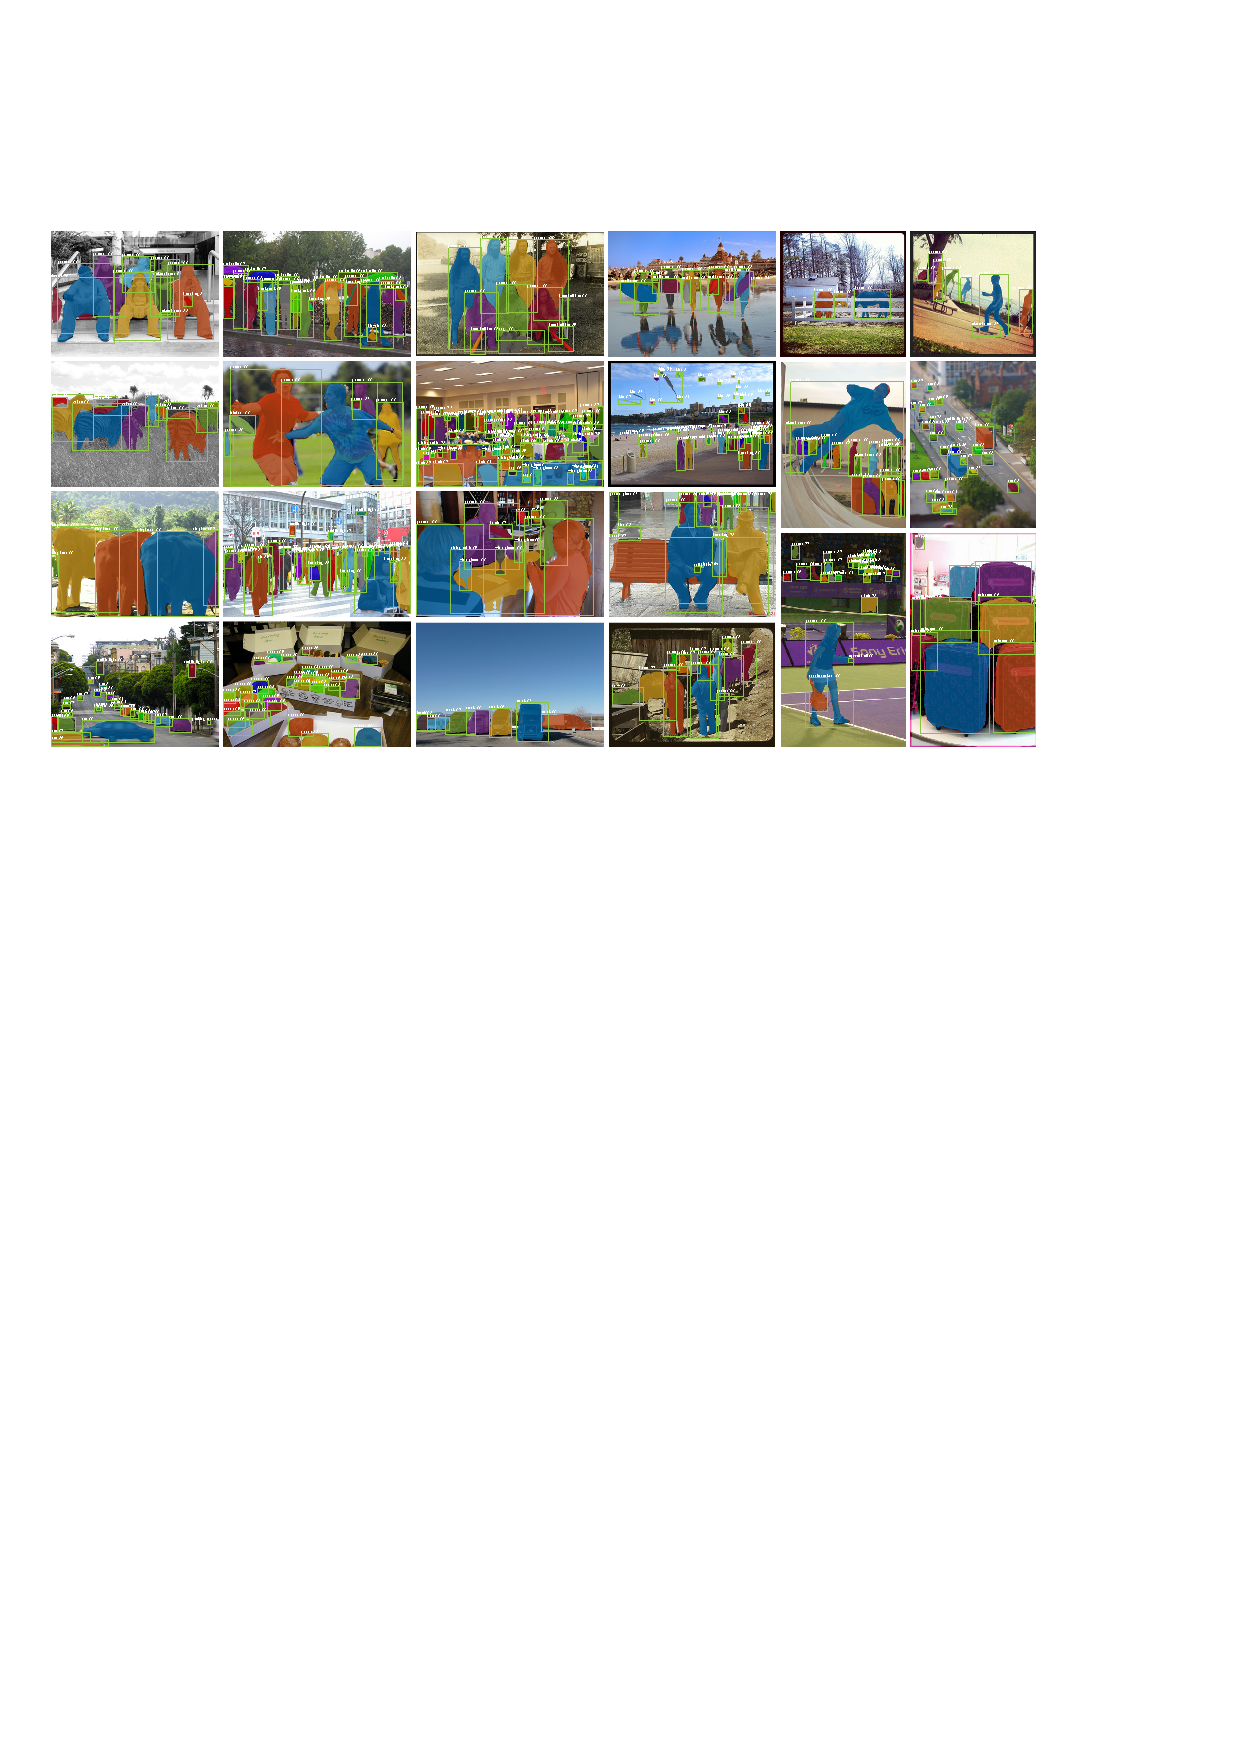
\includegraphics[width=1.0\linewidth]{figures/mask_rcnn/results_more}
\caption{More results of \textbf{Mask R-CNN} on COCO test images, using ResNet-101-FPN and running at 5 fps, with 35.7 mask AP (Table~\ref{tab:final_mask}).}
\label{fig:results_more}
\end{figure*}

\begin{table*}[t]
\tablestyle{3.5pt}{1.1}
\begin{tabular}{l|l|x{22}x{22}x{22}|x{22}x{22}x{22}}
  & backbone &  AP &  AP$_{50}$ & AP$_{75}$ & AP$_S$ &  AP$_M$ &  AP$_L$\\
\shline
  MNC  & ResNet-101-C4
  & 24.6 & 44.3 & 24.8 & 4.7 & 25.9 & 43.6\\
  FCIS  +OHEM & ResNet-101-C5-dilated
  & 29.2 & 49.5 & - & 7.1 & 31.3 & 50.0\\
  FCIS+++  +OHEM & ResNet-101-C5-dilated
  & 33.6 & 54.5 & - & - & - & -\\
\hline
  \textbf{Mask R-CNN} & ResNet-101-C4
  & 33.1 & 54.9 & 34.8 & 12.1 & 35.6 & 51.1 \\
  \textbf{Mask R-CNN} & ResNet-101-FPN
  & 35.7 & 58.0 & 37.8 & 15.5 & 38.1 & 52.4\\
  \textbf{Mask R-CNN} & ResNeXt-101-FPN
  & \textbf{37.1} & \textbf{60.0} & \textbf{39.4} & \textbf{16.9} & \textbf{39.9} & \textbf{53.5}
\end{tabular}
\caption{\textbf{Instance segmentation} \emph{mask} AP on COCO \texttt{test-dev}. MNC and FCIS are the winners of the COCO 2015 and 2016 segmentation challenges, respectively. Without bells and whistles, Mask R-CNN outperforms the more complex FCIS+++, which includes multi-scale train/test, horizontal flip test, and OHEM. All entries are \emph{single-model} results.}
\label{tab:final_mask}
\end{table*}

We adopt image-centric training. Images are resized such that their scale (shorter edge) is 800 pixels. Each mini-batch has 2 images per GPU and each image has $N$ sampled RoIs, with a ratio of 1:3 of positive to negatives. $N$ is 64 for the C4 backbone (as in) and 512 for FPN (as in).  We train on 8 GPUs (so effective mini-batch size is 16) for 160k iterations, with a learning rate of 0.02 which is decreased by 10 at the 120k iteration. We use a weight decay of 0.0001 and momentum of 0.9. With ResNeXt, we train with 1 image per GPU and the same number of iterations, with a starting learning rate of 0.01.

The RPN anchors span 5 scales and 3 aspect ratios, following. For convenient ablation, RPN is trained separately and does not share features with Mask R-CNN, unless specified. For every entry in this paper, RPN and Mask R-CNN have the same backbones and so they are shareable.

\paragraph{Inference:} At test time, the proposal number is 300 for the C4 backbone (as in) and 1000 for FPN (as in). We run the box prediction branch on these proposals, followed by non-maximum suppression. The mask branch is then applied to the highest scoring 100 detection boxes. Although this differs from the parallel computation used in training, it speeds up inference and improves accuracy (due to the use of fewer, more accurate RoIs). The mask branch can predict $K$ masks per RoI, but we only use the $k$-th mask, where $k$ is the predicted class by the classification branch. The $m \times m$ floating-number mask output is then resized to the RoI size, and binarized at a threshold of 0.5.

Note that since we only compute masks on the top 100 detection boxes, Mask R-CNN adds a small overhead to its Faster R-CNN counterpart (e.g., \app20\% on typical models).

\xjtuappendixsection{Experiments: Instance Segmentation}\label{sec:results}

We perform a thorough comparison of Mask R-CNN to the state of the art along with comprehensive ablations on the COCO dataset. We report the standard COCO metrics including AP (averaged over IoU thresholds), AP$_{50}$, AP$_{75}$, and AP$_S$, AP$_M$, AP$_L$ (AP at different scales). Unless noted, AP is evaluating using \emph{mask} IoU. As in previous work, we train using the union of 80k train images and a 35k subset of val images (\texttt{trainval35k}), and report ablations on the remaining 5k val images (\texttt{minival}). We also report results on \texttt{test-dev}.

\xjtuappendixsubsection{Main Results}

\begin{figure*}[t]
\centering
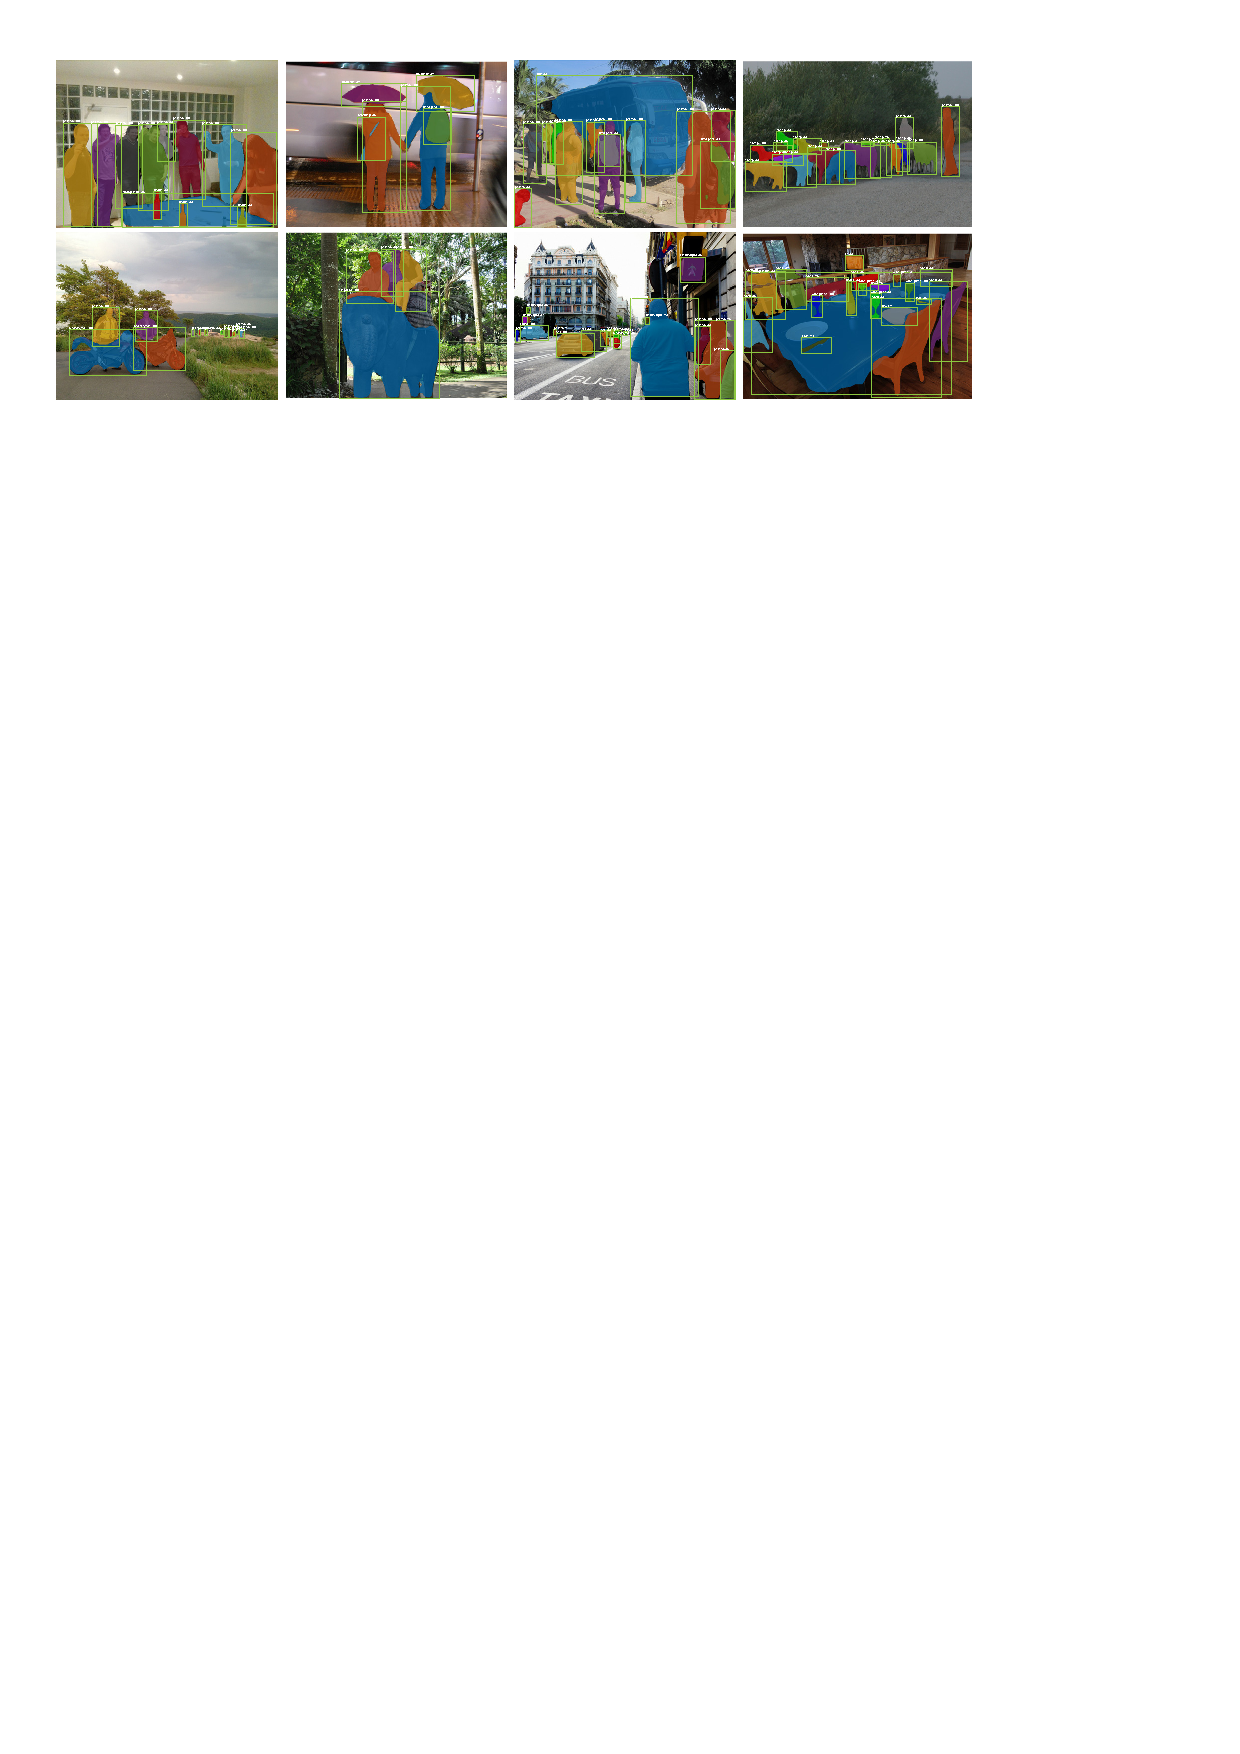
\includegraphics[width=1\linewidth]{figures/mask_rcnn/results_main}
\caption{\textbf{Mask R-CNN} results on the COCO test set. These results are based on ResNet-101, achieving a \emph{mask} AP of 35.7 and running at 5 fps. Masks are shown in color, and bounding box, category, and confidences are also shown.}
\label{fig:results_main}\vspace{-2mm}
\end{figure*}

We compare Mask R-CNN to the state-of-the-art methods in instance segmentation in Table \ref{tab:final_mask}. All instantiations of our model outperform baseline variants of previous state-of-the-art models. This includes MNC and FCIS, the winners of the COCO 2015 and 2016 segmentation challenges, respectively. Without bells and whistles, Mask R-CNN with ResNet-101-FPN backbone outperforms FCIS+++, which includes multi-scale train/test, horizontal flip test, and online hard example mining (OHEM). While outside the scope of this work, we expect many such improvements to be applicable to ours.

Mask R-CNN outputs are visualized in Figures \ref{fig:results_main} and \ref{fig:results_more}. Mask R-CNN achieves good results even under challenging conditions. In Figure \ref{fig:results_vs_fcis} we compare our Mask R-CNN baseline and FCIS+++. FCIS+++ exhibits systematic artifacts on overlapping instances, suggesting that it is challenged by the fundamental difficulty of instance segmentation. Mask R-CNN shows no such artifacts.

\begin{figure*}[t]
\centering
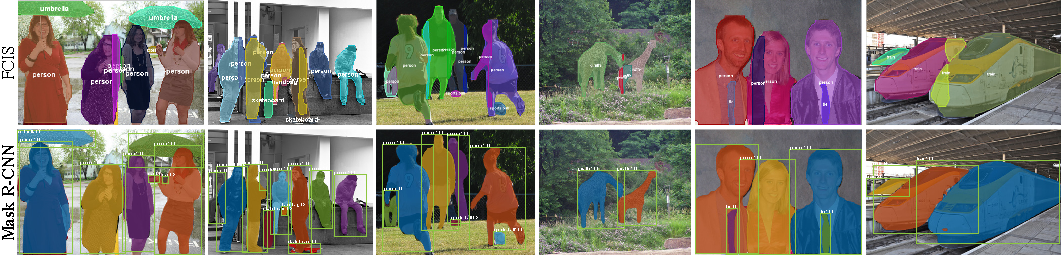
\includegraphics[width=1.0\linewidth]{figures/mask_rcnn/results_vs_fcis}
\caption{FCIS+++ (top) vs. Mask R-CNN (bottom, ResNet-101-FPN). FCIS exhibits systematic artifacts on overlapping objects.}
\label{fig:results_vs_fcis}
\end{figure*}

\begin{table*}[t]
% subfloat a - BackBone Architecture
\subfloat[\textbf{Backbone Architecture}: Better backbones bring expected gains: deeper networks do better, FPN outperforms C4 features, and ResNeXt improves on ResNet.\label{tab:ablation:backbone}]{
\tablestyle{2.5pt}{1.05}\begin{tabular}{c|x{22}x{22}x{22}}
  \scriptsize \emph{net-depth-features} & AP & AP$_{50}$ & AP$_{75}$\\
\shline
  \scriptsize ResNet-50-C4 & 30.3 & 51.2 & 31.5\\
  \scriptsize ResNet-101-C4 & 32.7 & 54.2 & 34.3\\\hline
  \scriptsize ResNet-50-FPN & 33.6 & 55.2 & 35.3\\
  \scriptsize ResNet-101-FPN & 35.4 & 57.3 & 37.5\\
  \scriptsize ResNeXt-101-FPN & \textbf{36.7} & \textbf{59.5} & \textbf{38.9}
\end{tabular}}\hspace{1mm}
% subfloat b - Multinomial vs Independent Masks
\subfloat[\textbf{Multinomial vs. Independent Masks} (ResNet-50-C4): \emph{Decoupling} via per-class binary masks (sigmoid) gives large gains over multinomial masks (softmax).\label{tab:ablation:sigmoid}]{
\tablestyle{4.8pt}{1.05}\begin{tabular}{c|x{22}x{22}x{22}}
  & AP & AP$_{50}$ & AP$_{75}$\\
\shline
  \emph{softmax} & 24.8 & 44.1 & 25.1\\
  \emph{sigmoid} & \textbf{30.3} & \textbf{51.2} & \textbf{31.5}\\
\hline
  & \dt{+5.5} & \dt{+7.1} & \dt{+6.4}\\
  \multicolumn{4}{c}{~}\\
  \multicolumn{4}{c}{~}\\
\end{tabular}}\hspace{1mm}
% subfloat c - RoIAlign (ResNet-50-C4)
\subfloat[\textbf{RoIAlign} (ResNet-50-C4): Mask results with various RoI layers. Our RoIAlign layer improves AP by $\app$3 points and AP$_{75}$ by $\app$5 points. Using proper alignment is the only factor that contributes to the large gap between RoI layers.\label{tab:ablation:roialign}]{
\tablestyle{2.2pt}{1.05}\begin{tabular}{c|c|c|c|x{22}x{22}x{22}}
  & \scriptsize\textbf{align?} & \scriptsize bilinear? & \scriptsize agg.
  & AP & AP$_{50}$ & AP$_{75}$\\
\shline
  \emph{RoIPool}
  & & & max & 26.9 & 48.8 & 26.4\\
\hline
  \multirow{2}{*}{\emph{RoIWarp} }
  & & \checkmark & max & 27.2 & 49.2 & 27.1\\
  & & \checkmark & ave & 27.1 & 48.9 & 27.1\\
\hline
  \multirow{2}{*}{\emph{RoIAlign}}
  & \checkmark & \checkmark & max & \textbf{30.2} & \textbf{51.0} & \textbf{31.8}\\
  & \checkmark & \checkmark & ave & \textbf{30.3} & \textbf{51.2} & \textbf{31.5}
\end{tabular}}\\
% subfloat d - RoIAlign (ResNet-50-C5)
\subfloat[\textbf{RoIAlign} (ResNet-50-\textbf{C5}, \emph{stride 32}): Mask-level and box-level AP using \emph{large-stride} features. Misalignments are more severe than with stride-16 features (Table \ref{tab:ablation:roialign}), resulting in big accuracy gaps.\label{tab:ablation:roialign32}]{
\tablestyle{4pt}{1.05}\begin{tabular}{c|x{22}x{22}x{22}|x{22}x{22}x{22}}
  & AP & AP$_{50}$ & AP$_{75}$
  & AP$^\text{bb}$ & AP$^\text{bb}_{50}$ & AP$^\text{bb}_{75}$ \\[.1em]
\shline
  \emph{RoIPool} & 23.6 & 46.5 & 21.6 & 28.2 & 52.7 & 26.9\\
  \emph{RoIAlign} & \textbf{30.9} & \textbf{51.8} & \textbf{32.1} & \textbf{34.0} & \textbf{55.3} & \textbf{36.4}\\
\hline
  & \dt{+7.3} & \dt{+ 5.3} & \dt{+10.5} & \dt{+5.8} & \dt{+2.6} & \dt{+9.5}
\end{tabular}}\hspace{2mm}
% subfloat e - mask representation
\subfloat[\textbf{Mask Branch} (ResNet-50-FPN): Fully convolutional networks (FCN) vs. multi-layer perceptrons (MLP, fully-connected) for mask prediction. FCNs improve results as they take advantage of explicitly encoding spatial layout.\label{tab:ablation:maskhead}]{
\tablestyle{4pt}{1.05}\begin{tabular}{c|c|x{22}x{22}x{22}}
  & mask branch & AP & AP$_{50}$ & AP$_{75}$\\
\shline
  MLP & fc: 1024$\rightarrow$1024$\rightarrow$$80\ncdot28^2$  & 31.5 & 53.7 & 32.8\\
  MLP & fc: 1024$\rightarrow$1024$\rightarrow$1024$\rightarrow$$80\ncdot28^2$ & 31.5 & 54.0 & 32.6\\
\hline
  \textbf{FCN} &  conv: 256$\rightarrow$256$\rightarrow$256$\rightarrow$256$\rightarrow$256$\rightarrow$80
  & \textbf{33.6} & \textbf{55.2} & \textbf{35.3}
\end{tabular}}
% main caption
\caption{\textbf{Ablations}. We train on \texttt{trainval35k}, test on \texttt{minival}, and report \emph{mask} AP unless otherwise noted.}
\label{tab:ablations}
\end{table*}

\xjtuappendixsubsection{Ablation Experiments}\label{sec:ablations}

We run a number of ablations to analyze Mask R-CNN. Results are shown in Table \ref{tab:ablations} and discussed in detail next.

\paragraph{Architecture:} Table \ref{tab:ablation:backbone} shows Mask R-CNN with various backbones. It benefits from deeper networks (50 vs.~101) and advanced designs  including FPN and ResNeXt. We note that \emph{not} all frameworks automatically benefit from deeper or advanced networks (see benchmarking in).

\paragraph{Multinomial vs. Independent Masks:} Mask R-CNN \emph{decouples} mask and class prediction: as the existing box branch predicts the class label, we generate a mask for each class without competition among classes (by a per-pixel \emph{sigmoid} and a \emph{binary} loss). In Table \ref{tab:ablation:sigmoid}, we compare this to using a per-pixel \emph{softmax} and a \emph{multinomial} loss (as commonly used in FCN). This alternative \emph{couples} the tasks of mask and class prediction, and results in a severe loss in mask AP (5.5 points). This suggests that once the instance has been classified as a whole (by the box branch), it is sufficient to predict a binary mask without concern for the categories, which makes the model easier to train.

\paragraph{Class-Specific vs. Class-Agnostic Masks:} Our default instantiation predicts class-specific masks, i.e., one $m \times m$ mask per class. Interestingly, Mask R-CNN with class-agnostic masks (i.e., predicting a single $m \times m$ output regardless of class) is nearly as effective: it has 29.7 mask AP vs. 30.3 for the class-specific counterpart on ResNet-50-C4. This further highlights the division of labor in our approach which largely decouples classification and segmentation.

\begin{table*}[t]
\tablestyle{3.5pt}{1.1}
\begin{tabular}{l|l|x{22}x{22}x{22}|x{22}x{22}x{22}}
  & backbone
  & AP$^\text{bb}$ & AP$^\text{bb}_{50}$ & AP$^\text{bb}_{75}$
  & AP$^\text{bb}_S$ & AP$^\text{bb}_M$ &  AP$^\text{bb}_L$\\ [.1em]
\shline
  Faster R-CNN+++  & ResNet-101-C4
  & 34.9 & 55.7 & 37.4 & 15.6 & 38.7 & 50.9\\
  Faster R-CNN w FPN  & ResNet-101-FPN
  & 36.2 & 59.1 & 39.0 & 18.2 & 39.0 & 48.2\\
  Faster R-CNN by G-RMI  & Inception-ResNet-v2
  & 34.7 & 55.5 & 36.7 & 13.5 & 38.1 & 52.0\\
  Faster R-CNN w TDM  & Inception-ResNet-v2-TDM
  & 36.8 & 57.7 & 39.2 & 16.2 & 39.8 & \textbf{52.1}\\
\hline
  Faster R-CNN, RoIAlign & ResNet-101-FPN
  & 37.3 & 59.6 & 40.3 & 19.8 & 40.2 & 48.8\\
  \textbf{Mask R-CNN} & ResNet-101-FPN
  & 38.2 & 60.3 & 41.7 & 20.1 & 41.1 & 50.2\\
  \textbf{Mask R-CNN} & ResNeXt-101-FPN
  & \textbf{39.8} & \textbf{62.3} & \textbf{43.4} & \textbf{22.1} & \textbf{43.2} & {51.2}
\end{tabular}
\caption{\textbf{Object detection} \emph{single-model} results (bounding box AP), vs. state-of-the-art on \texttt{test-dev}. Mask R-CNN using ResNet-101-FPN outperforms the base variants of all previous state-of-the-art models (the mask output is ignored in these experiments). The gains of Mask R-CNN over come from using RoIAlign (+1.1 AP$^\text{bb}$), multitask training (+0.9 AP$^\text{bb}$), and ResNeXt-101 (+1.6 AP$^\text{bb}$).}
\label{tab:final_bbox}
\end{table*}

\paragraph{RoIAlign:} An evaluation of our proposed \emph{RoIAlign} layer is shown in Table~\ref{tab:ablation:roialign}. For this experiment we use the ResNet-50-C4 backbone, which has stride 16. RoIAlign improves AP by about 3 points over RoIPool, with much of the gain coming at high IoU (AP$_{75}$). RoIAlign is insensitive to max/average pool; we use average in the rest of the paper.

Additionally, we compare with \emph{RoIWarp} proposed in MNC that also adopt bilinear sampling. As discussed in \S\ref{sec:maskrcnn}, RoIWarp still quantizes the RoI, losing alignment with the input. As can be seen in Table \ref{tab:ablation:roialign}, RoIWarp performs on par with RoIPool and much worse than RoIAlign. This highlights that proper alignment is key.

We also evaluate RoIAlign with a \emph{ResNet-50-C5} backbone, which has an even larger stride of 32 pixels. We use the same head as in Figure \ref{fig:head} (right), as the res5 head is not applicable. Table \ref{tab:ablation:roialign32} shows that RoIAlign improves mask AP by a massive 7.3 points, and mask AP$_{75}$ by 10.5 points (\emph{50\% relative improvement}). Moreover, we note that with RoIAlign, using \emph{stride-32} C5 features (30.9 AP) is more accurate than using stride-16 C4 features (30.3 AP, Table~\ref{tab:ablation:roialign}). RoIAlign largely resolves the long-standing challenge of using large-stride features for detection and segmentation.

Finally, RoIAlign shows a gain of 1.5 mask AP and 0.5 box AP when used with FPN, which has finer multi-level strides. For keypoint detection that requires finer alignment, RoIAlign shows large gains even with FPN (Table~\ref{tab:roialign_keypoint}).

\paragraph{Mask Branch:} Segmentation is a pixel-to-pixel task and we exploit the spatial layout of masks by using an FCN. In Table \ref{tab:ablation:maskhead}, we compare multi-layer perceptrons (MLP) and FCNs, using a ResNet-50-FPN backbone. Using FCNs gives a 2.1 mask AP gain over MLPs. We note that we choose this backbone so that the conv layers of the FCN head are not pre-trained, for a fair comparison with MLP.

\xjtuappendixsubsection{Bounding Box Detection Results}

We compare Mask R-CNN to the state-of-the-art COCO \emph{bounding-box} object detection in Table~\ref{tab:final_bbox}. For this result, even though the full Mask R-CNN model is trained, only the classification and box outputs are used at inference (the mask output is ignored). Mask R-CNN using ResNet-101-FPN outperforms the base variants of all previous state-of-the-art models, including the single-model variant of G-RMI, the winner of the COCO 2016 Detection Challenge. Using ResNeXt-101-FPN, Mask R-CNN further improves results, with a margin of 3.0 points box AP over the best previous single model entry from (which used Inception-ResNet-v2-TDM).

As a further comparison, we trained a version of Mask R-CNN but \emph{without} the mask branch, denoted by ``Faster R-CNN, RoIAlign'' in Table \ref{tab:final_bbox}. This model performs better than the model presented in due to RoIAlign. On the other hand, it is 0.9 points box AP lower than Mask R-CNN. This gap of Mask R-CNN on box detection is therefore due solely to the benefits of multi-task training.

Lastly, we note that Mask R-CNN attains a small gap between its mask and box AP: e.g., 2.7 points between 37.1 (mask, Table~\ref{tab:final_mask}) and 39.8 (box, Table~\ref{tab:final_bbox}). This indicates that our approach largely closes the gap between object detection and the more challenging instance segmentation task.

\xjtuappendixsubsection{Timing}

\paragraph{Inference:} We train a ResNet-101-FPN model that shares features between the RPN and Mask R-CNN stages, following the 4-step training of Faster R-CNN. This model runs at 195ms per image on an Nvidia Tesla M40 GPU (plus 15ms CPU time resizing the outputs to the original resolution), and achieves statistically the same mask AP as the unshared one. We also report that the ResNet-101-C4 variant takes $\app$400ms as it has a heavier box head (Figure \ref{fig:head}), so we do not recommend using the C4 variant in practice.

Although Mask R-CNN is fast, we note that our design is not optimized for speed, and better speed/accuracy trade-offs could be achieved, e.g., by varying image sizes and proposal numbers, which is beyond the scope of this paper.

\paragraph{Training:} Mask R-CNN is also fast to train. Training with ResNet-50-FPN on COCO \texttt{trainval35k} takes 32 hours in our synchronized 8-GPU implementation (0.72s per 16-image mini-batch), and 44 hours with ResNet-101-FPN. In fact, fast prototyping can be completed in \emph{less than one day} when training on the \texttt{train} set. We hope such rapid training will remove a major hurdle in this area and encourage more people to perform research on this challenging topic.

\begin{figure*}[t]
\centering
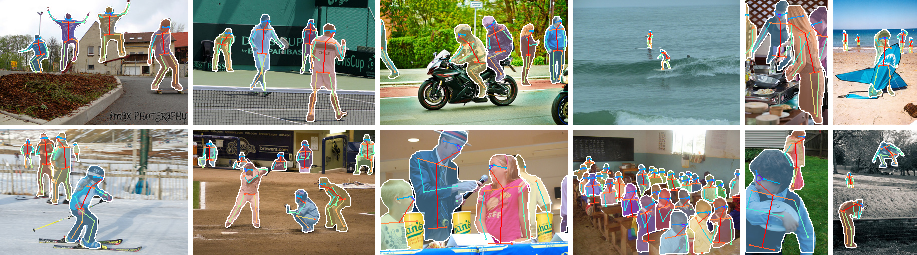
\includegraphics[width=1.0\linewidth]{figures/mask_rcnn/results_keypoints}
\caption{Keypoint detection results on COCO \texttt{test} using Mask R-CNN (ResNet-50-FPN), with person segmentation masks predicted from the same model. This model has a keypoint AP of 63.1 and runs at 5 fps.}
\label{fig:results_keypoints}
\end{figure*}

\xjtuappendixsection{Mask R-CNN for Human Pose Estimation}\label{sec:keypoints}

Our framework can easily be extended to human pose estimation. We model a keypoint's location as a one-hot mask, and adopt Mask R-CNN to predict $K$ masks, one for each of $K$ keypoint types (e.g., left shoulder, right elbow). This task helps demonstrate the flexibility of Mask R-CNN.

We note that \emph{minimal} domain knowledge for human pose is exploited by our system, as the experiments are mainly to demonstrate the generality of the Mask R-CNN framework. We expect that domain knowledge (e.g., modeling structures) will be complementary to our simple approach.

\paragraph{Implementation Details:} We make minor modifications to the segmentation system when adapting it for keypoints. For each of the $K$ keypoints of an instance, the training target is a one-hot $m \times m$ binary mask where only a \emph{single} pixel is labeled as foreground. During training, for each visible ground-truth keypoint, we minimize the cross-entropy loss over an $m^2$-way softmax output (which encourages a single point to be detected). We note that as in instance segmentation, the $K$ keypoints are still treated independently.

We adopt the ResNet-FPN variant, and the keypoint head architecture is similar to that in Figure \ref{fig:head} (right). The keypoint head consists of a stack of eight 3$\times$3 512-d conv layers, followed by a deconv layer and 2$\times$ bilinear upscaling, producing an output resolution of 56$\times$56. We found that a relatively high resolution output (compared to masks) is required for keypoint-level localization accuracy.

Models are trained on all COCO \texttt{trainval35k} images that contain annotated keypoints. To reduce overfitting, as this training set is smaller, we train using image scales randomly sampled from [640, 800] pixels; inference is on a single scale of 800 pixels. We train for 90k iterations, starting from a learning rate of 0.02 and reducing it by 10 at 60k and 80k iterations. We use bounding-box NMS with a threshold of 0.5. Other details are identical as in \S\ref{sec:impl}.

\begin{table}[t]
\tablestyle{1.8pt}{1.2}
\begin{tabular}{l|x{22}x{22}x{22}|x{22}x{22}}
  & AP$^\text{kp}$ & AP$^\text{kp}_{50}$ & AP$^\text{kp}_{75}$
  & AP$^\text{kp}_M$ &  AP$^\text{kp}_L$\\ [.1em]
\shline
CMU-Pose+++  & 61.8 & 84.9 & 67.5 & 57.1 & 68.2 \\
G-RMI $^\dagger$ & 62.4 & 84.0 & 68.5 & \textbf{59.1} & 68.1 \\
\hline
  \textbf{Mask R-CNN}, \footnotesize keypoint-only & 62.7 & 87.0 & 68.4 & 57.4 & 71.1 \\
  \textbf{Mask R-CNN}, \footnotesize keypoint \& mask & \textbf{63.1} & \textbf{87.3} & \textbf{68.7} & {57.8} & \textbf{71.4} \\
\end{tabular}
\caption{\textbf{Keypoint detection} AP on COCO \texttt{test-dev}. Ours is a single model (ResNet-50-FPN) that runs at 5 fps. CMU-Pose+++ is the 2016 competition winner that uses multi-scale testing, post-processing with CPM, and filtering with an object detector, adding a cumulative $\app$5 points (clarified in personal communication). $^\dagger$: G-RMI was trained on COCO \emph{plus} MPII (25k images), using two models (Inception-ResNet-v2 for bounding box detection and ResNet-101 for keypoints).}
\label{tab:final_keypoint}
\end{table}

\paragraph{Main Results and Ablations:} We evaluate the person keypoint AP (AP$^\text{kp}$) and experiment with a ResNet-50-FPN backbone; more backbones will be studied in the appendix. Table~\ref{tab:final_keypoint} shows that our result (62.7 AP$^\text{kp}$) is 0.9 points higher than the COCO 2016 keypoint detection winner that uses a multi-stage processing pipeline (see caption of Table~\ref{tab:final_keypoint}). Our method is considerably simpler and faster.

\begin{table}[t]
\begin{minipage}{0.55\textwidth}
  \tablestyle{7pt}{1.1}
  \begin{tabular}{l|x{22}x{22}x{22}}
  & AP$^\text{bb}_\text{\emph{person}}$ & AP$^\text{mask}_\text{\emph{person}}$
  & AP$^\text{kp}$ \\ [.1em]
  \shline
  Faster R-CNN & 52.5 & - & - \\
  Mask R-CNN, mask-only & \textbf{53.6} & \textbf{45.8} & - \\
  Mask R-CNN, keypoint-only & 50.7 & - & 64.2 \\
  Mask R-CNN, keypoint \& mask & 52.0 & 45.1 & \textbf{64.7} \\
  \end{tabular}
  \caption{\textbf{Multi-task learning} of box, mask, and keypoint about the \emph{person} category, evaluated on \texttt{minival}. All entries are trained on the same data for fair comparisons. The backbone is ResNet-50-FPN. The entries with 64.2 and 64.7 AP on \texttt{minival} have \texttt{test-dev} AP of 62.7 and 63.1, respectively (see Table~\ref{tab:final_keypoint}).}
  \label{tab:multitask_keypoint}
\end{minipage}\hspace{3mm}
\begin{minipage}{0.4\textwidth}
  \tablestyle{2pt}{1.1}
  \begin{tabular}{l|x{22}x{22}x{22}|x{22}x{22}}
    & AP$^\text{kp}$ & AP$^\text{kp}_{50}$ & AP$^\text{kp}_{75}$
    & AP$^\text{kp}_M$ &  AP$^\text{kp}_L$\\ [.1em]
  \shline
    \emph{RoIPool} & 59.8 & 86.2 & 66.7 & 55.1 & 67.4 \\
    \emph{RoIAlign}~~~~ & \textbf{64.2} & \textbf{86.6} & \textbf{69.7} & \textbf{58.7} & \textbf{73.0} \\
  \end{tabular}
  \caption{\textbf{RoIAlign vs. RoIPool} for keypoint detection on \texttt{minival}. The backbone is ResNet-50-FPN.}
  \label{tab:roialign_keypoint}
\end{minipage}
\end{table}

More importantly, we have \emph{a unified model that can simultaneously predict boxes, segments, and keypoints} while running at 5 fps. Adding a segment branch (for the person category) improves the AP$^\text{kp}$ to 63.1 (Table~\ref{tab:final_keypoint}) on \texttt{test-dev}. More ablations of multi-task learning on \texttt{minival} are in Table~\ref{tab:multitask_keypoint}. Adding the \emph{mask} branch to the box-only (i.e., Faster R-CNN) or keypoint-only versions consistently improves these tasks. However, adding the keypoint branch reduces the box/mask AP slightly, suggesting that while keypoint detection benefits from multitask training, it does not in turn help the other tasks. Nevertheless, learning all three tasks jointly enables a unified system to efficiently predict all outputs simultaneously (Figure~\ref{fig:results_keypoints}).

We also investigate the effect of \emph{RoIAlign} on keypoint detection (Table~\ref{tab:roialign_keypoint}).  Though this ResNet-50-FPN backbone has finer strides (e.g., 4 pixels on the finest level), RoIAlign still shows significant improvement over RoIPool and increases AP$^\text{kp}$ by 4.4 points. This is because keypoint detections are more sensitive to localization accuracy. This again indicates that alignment is essential for pixel-level localization, including masks and keypoints.

Given the effectiveness of Mask R-CNN for extracting object bounding boxes, masks, and keypoints, we expect it be an effective framework for other instance-level tasks.

\begin{table*}[t]
\tablestyle{4pt}{1.05}
\begin{tabular}{l|l|x{32}|x{22}x{22}|x{22}x{22}x{22}x{22}x{22}x{22}x{22}x{22}}
  & \multicolumn{1}{c|}{training data} & AP [\texttt{val}] & AP & AP$_{50}$
  & person & rider & car & truck & bus & train & mcycle & bicycle\\[.1em]
\shline
  InstanceCut  & \texttt{fine} + \texttt{coarse}
  & 15.8 & 13.0 & 27.9 & 10.0 & 8.0 & 23.7 & 14.0 & 19.5 & 15.2 & 9.3 & 4.7 \\
  DWT  & \texttt{fine}
  & 19.8 & 15.6 & 30.0 & 15.1 & 11.7 & 32.9 & 17.1 & 20.4 & 15.0 & 7.9 & 4.9 \\
  SAIS  & \texttt{fine}
  & - & 17.4 & 36.7 & 14.6 & 12.9 & 35.7 & 16.0 & 23.2 & 19.0 & 10.3 & 7.8 \\
  DIN  & \texttt{fine} + \texttt{coarse}
  & - & 20.0 & 38.8 & 16.5 & 16.7 & 25.7 & 20.6 & 30.0 & 23.4 & 17.1 & 10.1 \\
  SGN  & \texttt{fine} + \texttt{coarse} & 29.2 & 25.0 & 44.9 & 21.8 &	20.1 &	39.4 &	24.8 &	33.2 &	30.8 &	17.7 &	12.4 \\
\hline
  Mask R-CNN & \texttt{fine}
  & 31.5 & 26.2 & 49.9 & 30.5 & 23.7 & 46.9 & 22.8 & 32.2 & 18.6 & 19.1 & 16.0 \\
  Mask R-CNN & \texttt{fine} + COCO
  & \textbf{36.4} & \textbf{32.0} & \textbf{58.1} & \textbf{34.8} & \textbf{27.0} & \textbf{49.1} & \textbf{30.1} & \textbf{40.9} & \textbf{30.9} & \textbf{24.1} & \textbf{18.7} \\
\end{tabular}
\caption{Results on Cityscapes \texttt{val} (`AP [\texttt{val}]' column) and \texttt{test} (remaining columns) sets. Our method uses ResNet-50-FPN.}
\label{tab:cityscapes}
\end{table*}